\chapter{Dynamic Behavior of the System}
\section{Steady States and their Stability}
\paragraph* {Equilibrium Points:}
The equilibrium points are generated using following set of equations and dynamics of the model is analysed using these set of points:
 $$ \frac{dS}{dt} = 0 = \frac{dL}{dt} = \frac{dB}{dt} = \frac{dR}{dt} = \frac{dA}{dt}=\frac{d{S_1}}{dt}=\frac{d{L_1}}{dt}= \frac{d{B_1}}{dt}=\frac{d{R_1}}{dt}=\frac{d{A_1}}{dt} $$
 from the system of targeted and attacker class equations.\\
System has sixteen equilibrium states. It has following four malicious codes-free equilibrium states:

$E_{1} = ( 1 , 0 , 0 , 0 , 0 , 1 , 0 , 0 , 0 , 0 ) \label{eq:E1},$

$E_{2} =  ( 1 , 0 , 0 , 0 , 0 ,  \frac{1+c_{1}}{k_{1}}  , 0 , 0 , 0 , 1 - \frac{1+c_{1}}{k_{1}})\label{eq:E2},$

$E_{3} =  ( \frac{1+c}{k} , 0 , 0 , 0 , 1-\frac{1+c}{k} , 1 , 0 , 0 , 0  ,0 )\label{eq:E3},$

$E_{4} =  ( \frac{1+c}{k} , 0 , 0 , 0 , 1-\frac{1+c}{k} , \frac{1+c_{1}}{k_{1}}  , 0 , 0 , 0 , 1 - \frac{1+c_{1}}{k_{1}})\label{eq:E4},$
%\begin{align}

%& E_{1} &= \left( 1,\ 0,\ 0,\ 0,\ 0,\ 1, \ 0, \ 0, \ 0, \ 0 \right), \label{eq:E1}\\

%& E_{2} &= \left( 1,\ 0,\ 0,\ 0,\ 0,\ \frac{1+c_1}{k_1}, \ 0, \ 0, \ 0, \ 1- \frac{1+c_1}{k_1} \right), \label{eq:E2}\\

%& E_{3} &= \left( \frac{1+c}{k},\ 0,\ 0,\ 0,\ 1- \frac{1+c}{k},\ 1, \ 0, \ 0, \ 0, \ 0 \right), \label{eq:E3}\\

%& E_{4} &= \left( \frac{1+c}{k},\ 0,\ 0,\ 0,\ 1- \frac{1+c}{k},\ \frac{1+c_1}{k_1}, \ 0, \ 0, \ 0, \ 1- \frac{1+c_1}{k_1} \right), \label{eq:E4}\\
%\end{align}
and twelve endemic equilibrium states:

$E_{5} =(1,0,0,0,0,\hat{S_1},0,\hat{B_1},\hat{R_1},\hat{A_1}) \label{eq:E5},$

$E_{6} =(1,0,0,0,0,\hat{S_1},\hat{L_1},\hat{B_1},\hat{R_1},\hat{A_1}) \label{eq:E6},$

$E_{7} =(\frac{1+c}{k},0,0,0,1-\frac{1+c}{k},\hat{S_1},0,\hat{B_1},\hat{R_1},\hat{A_1})\label{eq:E7},$

$E_{8} =(\frac{1+c}{k},0,0,0,1-\frac{1+c}{k},\hat{S_1},\hat{L_1},\hat{B_1},\hat{R_1},\hat{A_1})\label{eq:E8},$

$E_{9} =(\hat{S},0,\hat{B},\hat{R},\hat{A},1,0,0,0,0) \label{eq:E9},$

$E_{10} =(\hat{S},0,\hat{B},\hat{R},\hat{A},\frac{1+c_1}{k_1},0,0,0,1-\frac{1+c_1}{k_1}) \label{eq:E10},$

$E_{11} =(\hat{S},0,\hat{B},\hat{R},\hat{A},\hat{S_1},0,\hat{B_1},\hat{R_1},\hat{A_1}) \label{eq:E11},$

$E_{12} =(\hat{S},0,\hat{B},\hat{R},\hat{A},\hat{S_1},\hat{L_1},\hat{B_1},\hat{R_1},\hat{A_1}) \label{eq:E12},$

$E_{13} =(\hat{S},\hat{L},\hat{B},\hat{R},\hat{A},1,0,0,0,0) \label{eq:E13},$

$E_{14} =(\hat{S},\hat{L},\hat{B},\hat{R},\hat{A},\frac{1+c_1}{k_1},0,0,0,1-\frac{1+c_1}{k_1}) \label{eq:E14},$

$E_{15} =(\hat{S},\hat{L},\hat{B},\hat{R},\hat{A},\hat{S_1},0,\hat{B_1},\hat{R_1},\hat{A_1}) \label{eq:E15},$

$E_{16} =(\hat{S},\hat{L},\hat{B},\hat{R},\hat{A},\hat{S_1},\hat{L_1} ,\hat{B_1},\hat{R_1},\hat{A_1}) \label{eq:E16}.$


\noindent Here we observed that the equilibrium point $E_1$ is on the $S-S_1$ plane and the equilibrium point  $E_2$ is on the $S-S_1-A_1$ plane. Also the equilibrium point $E_3$ is on the $S-A-S_1$ plane and the equilibrium point $E_4$ is on the $S-A-S_1-A_1$ plane in the space and all other equilibrium states are interior points on the space. Steady state $E_1$ is always feasible since all the other parameters are positive. State $E_2$, $E_3$ and $E_4$ are feasible when $\frac{1+c}{k} \leq 1$ and $\frac{1+c_{1}}{k_{1}} \leq 1.$ Numerical values of parameters are used to calculate the feasibility of other non-malicious code free steady states for different parameter sets.\\
The expressions for the equilibrium points are used to obtain the conditions for stability of malicious-code free solutions. To avoid infection propagation, it will be useful for obtaining the minimum recovery rate.

\section{Basic Reproduction Number}
Basic reproduction number, $R_{0}$ is defined by the expected number of secondary cases produced by a single infection in a completely susceptible population. To characterize the malicious object propagation, it is considered as one of the most useful threshold parameter. The derivative of infection classes, i.e., $2^{nd}$ and $3^{rd}$ equations of targeted system and $2^{nd}$ and $3^{rd}$ equations of attacker system.\\
Let $x$= $(L, B, L_{1}, B_{1})$, then

$\frac{dx}{dt} = \cal{F}-\cal{V},$

\noindent where,

$\cal{F}$ =
    ${\left(
    \begin{array}{c}
      {\beta}_2 e^{-m_1 B} S B+{\beta}_2 e^{-m_2 B_1} S B_1+B S \\
      {\beta}_1 e^{-m_1 L} S L+{\beta}_1 e^{-m_2 L_1} S L_1+L S  \\
      {\beta}_4 S_1 N_1 B_1+B_1 S_1 \\
      {\beta}_3 S_1 N_1 L_1+S_1 L_1 \\
    \end{array}
  \right) },$


 $\cal{V}$ =
 ${\left(
   \begin{array}{c}
     d_2 B -\varepsilon L +\gamma B +\frac{B}{N} -d_2 B^2 -B R - B A - d_2 B L \\
     d_2 L +\varepsilon L +\delta B +\frac{L}{N} -d_2 L^2 - R L - A L - d_2 B L \\
     d_3 B_1 - \varepsilon L_1+\gamma B_1 +\frac{B_1}{N_1}-d_3 L_1 B_1 -d_3 {B_1}^2 -B_1 R_1 -B_1 A_1 \\
     d_3 L_1 + \varepsilon L_1+\delta L_1 +\frac{L_1}{N_1}-d_3 L_1 B_1 -d_3 {L_1}^2 -L_1 R_1 -L_1 A_1 \\
   \end{array}
 \right)},$

 \noindent we get,

\noindent F(Jacobian of $\cal{F}$  at malicious codes-free equilibrium)=

     $\left(
       \begin{array}{cccc}
         ({\beta}_2+1) S & 0 & {\beta}_2 S & 0 \\
         0 & ({\beta}_1+1) S & 0 & {\beta}_1 S \\
         0 & 0 & ({\beta}_4+1) S_1 & 0 \\
         0 & 0 & 0 & ({\beta}_3+1) S_1 \\
       \end{array}
     \right),$

\noindent and,

\noindent V(Jacobian of $\cal{V}$  at malicious codes-free equilibrium)=

 $\left(
   \begin{array}{cccc}
     \gamma-A+d_2+1 & -\varepsilon & 0 & 0 \\
     0 & \varepsilon-A+\delta+d_2+1 & 0 & 0 \\
     0 & 0 & {\gamma}_1-A_1+d_3+1 & -{\varepsilon}_1 \\
     0 & 0 & 0 & d_3-A_1+{\varepsilon}_1+{\delta}_1+1 \\
   \end{array}
 \right).$

F is the rate matrix of secondary infection and V is the rate matrix of the transmission. Then, the dominant eigenvalue of $FV^{-1}$ is called the basic reproductive number $R_0$.

$R_0 = max\left\{\frac{S(1+{\beta}_1)}{1+d_2+\delta+\varepsilon-A},\frac{S_1(1+{\beta}_3)}{1+d_3+{\delta}_1+{\varepsilon}_1-A_1},
\frac{S(1+{\beta}_2)}{1+d_2+\gamma-A},\frac{S_1(1+{\beta}_4)}{1+d_3+{\gamma}_1-A_1}\right\},$

\noindent where $S, S_1$ is the node density of susceptible class and $A, A_1$ is the node density of antidotal class of targeted and attacker population respectively in malicious codes - free equilibrium state. This model has four such states $E_1, E_2, E_3$ and $E_4$ and hence we have four basic reproduction number $R_{01}, R_{02}, R_{03}$ and $R_{04}$ respectively.
Value of $R_{01}, R_{02}, R_{03}$ and $R_{04}$ are:

\noindent for equilibrium state $E_1:$\\
$S=1,A=0,S_1=1,A_1=0$ and hence,

$R_{01}$=$max$\{$\frac{1+{\beta}_1}{1+d_2+\delta+\varepsilon}$,$\frac{1+{\beta}_3}{1+d_3+{\delta}_1+{\varepsilon}_1}$,$\frac{1+{\beta}_2}{1+d_2+\gamma}$,
$\frac{1+{\beta}_4}{1+d_3+{\gamma}_1}$\}.\\

\noindent Similarly for $E_2:$\\
$S=1,A=0,S1=\frac{1+c_1}{k_1},A_1=1-\frac{1+c_1}{k_1}$ and hence,

$R_{02}$=$max$\{$\frac{1+{\beta}_1}{1+d_2+\delta+\varepsilon}$,$\frac{(1+c_1)(1+{\beta}_3)}{(k_1)(1+d_3+{\delta}_1+{\varepsilon}_1\frac{1+c_1}{k_1})}$,
$\frac{1+{\beta}_2}{1+d_2+\gamma}$,$\frac{(1+{\beta}_4)(1+c_1)}{(k_1)(1+d_3+{\gamma}_1+\frac{1+c_1}{k_1})}$\}.\\

\noindent Similarly for $E_3:$\\
$S=\frac{1+c}{k}, A_1=1-\frac{1+c}{k},S1=\frac{1+c_1}{k_1},A_1=1-\frac{1+c_1}{k_1}$ and hence,

$R_{03}$=$max$\{$\frac{(1+{\beta}_1)(1+c)}{(k)(\frac{1+c}{k}+d_2+\delta+\varepsilon)}$,$\frac{(1+c_1)(1+{\beta}_3)}{(k_1)(1+d_3+{\delta}_1+{\varepsilon}_1\frac{1+c_1}{k_1})}$,
$\frac{(1+{\beta}_2)(1+c)}{(k)(\frac{1+c}{k}+d_2+\gamma)}$,$\frac{(1+{\beta}_4)(1+c_1)}{(k_1)(1+d_3+{\gamma}_1+\frac{1+c_1}{k_1})}$\}.\\

\noindent Similarly for $E_4:$\\
$S=\frac{1+c}{k},A_1=1-\frac{1+c}{k},S1=1,A_1=0$ and hence,

$R_{04}$=$max$\{$\frac{(1+{\beta}_1)(1+c)}{(k)(\frac{1+c}{k}+d_2+\delta+\varepsilon)}$,$\frac{(1+{\beta}_3)}{1+d_3+{\delta}_1+{\varepsilon}_1}$,
$\frac{(1+{\beta}_2)(1+c)}{(k)(\frac{1+c}{k}+d_2+\gamma)}$,$\frac{(1+{\beta}_4)}{1+d_3+{\gamma}_1}$\}.

\section{Local Asymptotical Stability}

We define the local asymptotic stability of malicious codes-free and endemic equilibrium.\\
\noindent Jacobian matrix which is applicable for all the equilibrium points is given below:

\noindent
\begin{math}
\small\left(
        \begin{array}{llllllllll}
           a_1& a_2 & a_3 &  & a_5 & 0 &-S \beta_{1} &-S \beta_{2} & 0 & 0 \\
          0 &  & 0 & 0 & 0 & 0  & S \beta_{1} & 0 & 0 & 0\\
          0 & \epsilon & a_7 & 0 & 0 & 0 & 0 & 0 & 0 & S \beta_{2} \\
          0 & \delta & \gamma & a_8 & 0 & 0 & 0 & 0 & 0 & 0 \\
          2A+Ak(1+S) & a_9 & a_{10} & a_{11} & a_{12} & 0 & 0 & 0 & 0 & 0 \\
          0 & 0 & 0 & 0 & 0 & a_{13} & a_{14} & a_{15} & a_{16} & a_{17}  \\
          0 & 0 & 0 & 0 & 0 & 0 & a_{18} & 0 & 0 & 0 \\
          0 & 0 & 0 & 0 & 0 & 0 & \epsilon_{1} & a_{19} & 0 & 0  \\
          0 & 0 & 0 & 0 & 0 & 0 & \delta_{1} & \gamma_{1} & a_{20} & 0  \\
          0 & 0 & 0 & 0 & 0 & a_{21} & a_{22} & a_{23} & a_{24} & a_{25}  \\
        \end{array}
      \right)\normalsize
\end{math}

\noindent where,\\
\noindent $a_1=3+A+3S- k A (1+S)$,\\
$a_2=-1+S+d_{2} S-  k A S- \beta_{1} S$,\\
$a_3=-1+S+d_{2} S-  k A S- \beta_{2} S$,\\
$a_4=-1+2S- k A S+\alpha$,\\
$a_5=-1+c+2S-k (1+A) S$,\\
$a_6=-1+A-d_{2}+S+ \beta_{1} S-\delta -\epsilon$,\\
$a_7=-d_{2}+\beta_{2} S-\gamma-1+A+S$,\\
$a_8=-2+A-f+S-\alpha$,\\
$a_9=A+d_{2} A+k A S$;  $a_{10}=A+d_{2} A+k A S$,\\
$a_{11}=2A+f+k A S$;  $a_{12}=-2+3A-c+S+k (1+A) S$,\\
$a_{13}=-3+A_{1}- k_{1} A_{1}+3 S_{1}- k_{1} A_{1} S_{1}$,\\
$a_{14}=-1+S_{1}+d_{3} S_{1}- k_{1} A_{1} S_{1}-\beta_{3} S_{1}$,\\
$a_{15}=-1+S_{1}+d_{3} S_{1}-k_{1} A_{1}  S_{1}-\beta_{4} S_{1}$,\\
$a_{16}=-1+2 S_{1}-k_{1} A_{1} S_{1}+\alpha_{1}$,\\
$a_{17}=-1+c_{1}+2 S_{1}-k_{1}  (1+A_{1}) S_{1}$,\\
$a_{18}=-1+A_{1}+S_{1}+\beta_{3} S_{1}-d_{3} - \delta{1} - \epsilon_{1}$,\\
$a_{19}=-1+A_{1}-d_{3} +S_{1}+ \beta_{3} S_{1} - \delta_{1}-\epsilon_{1}$,\\
$a_{20}=-2+A_{1}-f_{1}+S_{1}-\alpha_{1}$,\\
$a_{21}=2 A_{1}+ k_{1} A_{1}+k_{1} A_{1} S_{1}$,\\
$a_{22}=A_{1}+d_{3} A_{1}+ k_{1} A_{1} S_{1}$,\\
$a_{23}=A_{1}+d_{3} A_{1}+k_{1} A_{1} S_{1}$,\\
$a_{24}=2 A_{1}+f_{1}+ k_{1} A_{1} S_{1}$,\\
$a_{25}=-2+3 A_{1}-c_{1}+S_{1}+k_{1} S_{1}+  k_{1} A_{1} S_{1}.$\\

\noindent At malicious codes - free equilibrium, the variational matrix $E_1$ is as follows:\\

\noindent
\begin{math}
\small\left(
%{\scriptsize{
        \begin{array}{llllllllll}
          0 & a_1 & d_{2} - \beta_{2} & 1 + \alpha & a_3 & 0 & - \beta_{1} & - \beta_{2} & 0 & 0 \\
          0 & a_2 & 0 & 0 & 0 & 0  & \beta_{1} & 0 & 0 & 0\\
          0 & \epsilon & a_5 & 0 & 0 & 0 & 0 & \beta_{2} & 0 & 0 \\
          0 & \delta & \gamma & -1-f-\alpha & 0 & 0 & 0 & 0 & 0 & 0 \\
          0 & 0 & 0 & 0 & f & a_4 & 0 & 0 & 0 & 0 \\
          0 & 0 & 0 & 0 & 0 & 0 & d_{3} - \beta_{3} & d_{3} - \beta_{4} & 1 + \alpha_{1} & a_6 \\
          0 & 0 & 0 & 0 & 0 & 0 & a_7 & 0 & 0 & 0 \\
          0 & 0 & 0 & 0 & 0 & 0 & \epsilon_{1} & -d_{3} + \beta_{4} - \gamma_{1} & 0 & 0  \\
          0 & 0 & 0 & 0 & 0 & 0 & \delta_{1} & \gamma_{1} & -1 - f{1} - \alpha_{1} & 0  \\
          0 & 0 & 0 & 0 & 0 & 0 & 0 & 0 & f{1} & a_8  \\
        \end{array}
%}}
      \right)\normalsize.
\end{math}

\noindent Where,\\
$a_1=d_{2} - \beta_{1}$, $a_2=-d_{2}+\beta_{1}-\delta-\epsilon$,
$a_3= 1 + c -k$,$a_4=- 1 - c - k_{0}$, $a_5=-d_{2}+\beta_{2}-\gamma$, $a_6=1 + c_{1} - k_{1}$, $a_7=-d_{3} + \beta_{3} - \delta{1} - \epsilon_{1}$, $a_8=- 1 - c_{1} - k_{1} S_{1}.$

\noindent The eigenvalues of this matrix are:
\noindent \[
\left\{0,0,0,-1-c+k,-1-f-\alpha,-1-f_{1}-\alpha_{1},-d_{2}+\beta_{2}-\gamma, -d_{3}+\beta_{4}-\gamma_{1},
  \right. \]
\[ \left. -d_{2}+\beta_{1}-\delta-\epsilon, -d_{3}+\beta_{3}-\delta_{1}-\epsilon_{1} \right\}. \]
\noindent Equilibrium state $E_1$ is said to be locally asymptotically stable when all  eigenvalues of $J_ {01}$ are having negative real parts or negative in nature.
So, if ${{\cal R}}_{01}<1$, then all the eigenvalues will have negative real parts. Hence, we can say the malicious code free equilibrium $E_1$ is locally asymptotically unstable, if ${\cal R}_{01} > 1$ and stable, if ${\cal R}_{01} < 1$.\\
Similarly, the eigenvalues of Jacobian matrix $J_{02}$ for malicious codes free equilibrium state $E_2$, are given by:
\[
\left\{0,-1-c+k,0,0,-(1 - \frac{1+c_{1}}{k_{1}}k_{1}),-1-f-\alpha,-1-f_{1}-\alpha_{1},-d_{2}+\beta_{2}-\gamma,
  \right. \]
\[ \left. -d_{3}+ \frac{(1+c_{1})(\beta_{4})}{k_{1}}-\gamma_{1},\\-d_{2}+\beta_{1}-\delta-\epsilon,-d_{3}+\frac{(\beta_{3})(1+c_{1})
}{k_{1}}-\delta_{1}-\epsilon_{1}\right\}, \]

\noindent which shows that if ${{\cal R}}_{02} < 1$, then $J_{02}$ will have negative real parts for all the eigenvalues. Hence, $E_2$ is locally asymptotically stable.\\
Similarly, the eigenvalues of Jacobian matrix $J_{03}$ for malicious codes free equilibrium state $E_3$, are given by,
\[
\left\{0,-{1-\frac{1+c}{k}} k,0,-(1-\frac{1+c_{1}}{k_{1}}) k_{1}, -1-f-\alpha,-1-f_{1}-\alpha_{1},-d_{2}+\frac{(\beta_{2})(1+c)}{k}-\gamma,
  \right. \]
\[ \left. -d_{3}+\frac{(1+c_{1})(\beta_{4})}{k_{1}}-\gamma_{1},\\
-d_{2}+\frac{\beta_{1}(1+c)}{k}-\delta-\epsilon,-d_{3}+\frac{\beta_{3}(1+c_{1})}{k_{1}}-\delta_{1}-\epsilon_{1}\right\}, \]

\noindent which shows that if ${{\cal R}}_{03} < 1$, then $J_{03}$ will have negative real parts for all the eigenvalues. Hence, $E_3$ is locally asymptotically stable.\\
Similarly, the eigenvalues of Jacobian matrix $J_{04}$ for malicious codes free equilibrium state $E_4$, are given by,
\[
\left\{0,-{1-\frac{1+c}{k}} k,0,-1-c_{1}+k_{1}, -1-f-\alpha,-1-f_{1}-\alpha_{1},-d_{2}+\frac{\beta_{2}(1+c)}{k}-\gamma,
  \right. \]
\[ \left. -d_{3}+\beta_{4}-\gamma_{1},
-d_{2}+\frac{\beta_{1}(1+c)}{k}-\delta-\epsilon,-d_{3}+\beta_{3}-\delta_{1}-\epsilon_{1}\right\}, \]

\noindent which shows that if ${{\cal R}}_{04} < 1$, then $J_{04}$ will have negative real parts for all the eigenvalues. Hence, $E_4$ is locally asymptotically stable.\\

\section{Numerical Simulation}
Numerical methods are used to solve the system of equations for the targeted and attacker system. For the different classes the behavior of the nodes is observed with respect to the time.
The targeted and attacker system has been solved and simulated and the behavior of the nodes in different classes are observed with respect to the time.
\subsection{Feasible Steady States}
For the model, for different parameter sets feasible steady states are simulated and analysed. At any point if all the classes have non-negative values, then a steady state is said to be feasible at this point. Following table \ref{T1} shows the feasibility of steady states with basic reproduction number and for different parameter set.

We plot a curve to understand the behavior of the classes with time. Figures show the node density of $S,L,B,R$ and $A$ nodes of attacker and targeted class. Since $E_{1}, E_{2},E_{3}$ and $E_{4}$ are the malicious code free states so they would be present in every set of equilibrium states if their reproduction number $R_{0}<1$, otherwise equilibrium will tend to some other states if their $R_{0}>1$. All observations are done with respect to the time and by using different parameter sets.

%\begin{figure}
%\centering
%\subfigure[Node Density vs. Time for different classes with various parameter sets and initial points for SLBRA model]{\label{fig:ff0}\includegraphics[width=0.8\columnwidth, clip=true]{6.eps}}
%\caption{Node Density vs. Time for different classes}
%\end{figure}
\noindent Figure \ref{fig:ff0} is plotted with parameter set 1 and initial point (0.5, 0.2, 0.25, 0, 0.05, 0.1, 0.35,0.4, 0.1, 0.05). In this figure at steady state node density of $S, B, R, A$ , $S_{1}$ and $A_{1}$ classes are greater than zero and possible feasible states are $E_{1}, E_{2}, E_{3}, E_{4}, E_{9}$ and $E_{10}$. Since all the reproduction number is greater than 1, hence we can conclude that $E_{10}$ is the stable steady state.

\noindent Figure \ref{fig:ff2} is plotted with parameter set 1 and initial point (0.52, 0.02, 0.025, 0.05, 0.43, 1, 0, 0, 0, and 0). Similarly, we can conclude that $E_{1}, E_{2}, E_{3}, E_{4}, E_{9}$ and $E_{10}$ are the feasible steady states and $E_{9}$ is the stable steady state.

\begin{table}
\centering
%\label{tab:equilibrium_SLBRA}
    \begin{tabular}{|p{1.9cm}|p{1.8cm}|p{1.8cm}|p{1.8cm}|p{1.8cm}|p{1.8cm}|p{1.8cm}|p{1.8cm}|}
    \hline
               Parameters      & \textbf{Set 1} & \textbf{Set 2} & \textbf{Set 3} & \textbf{Set 4} & \textbf{Set 5} & \textbf{Set 6} \\
            \hline
  $\boldsymbol {\beta_{1}} $                 & 0.6 & 0.6 & 0.7 & 1 & 0.87 & 0.73  \\
  $\boldsymbol {\beta_{2}} $     & 0.5 & 0.5 & 0.4 & 0.8 & 0.43 & 0.50 \\
  \textbf {k}      & 0.06 & 0.06 & 0.06 & 0.16 & 0.036 & 0.06\\
  \textbf{c}               & 0.03 & 0.03 & 0.03 & 0.08 & 0.06 & 0.03\\
  $\boldsymbol{\alpha}$         & 0.05 & 0.05 & 0.05 & 0.15 & 0.10 & 0.058 \\
  $\mathbf {d _{2} }$          & 0.04 & 0.08 & 0.1 & 0.1 & 0.121 & 0.25 \\
  $\boldsymbol{\epsilon}$         & 0.3 & 0.3 & 0.4 & 0.4 & 0.46 & 0.4 \\
  $\boldsymbol{\gamma}$                & 0.045 & 0.45 & 0.1 & 0.1 & 0.15 & 0.1\\
  $\boldsymbol{\delta}$       & 0.025 & 0.25 & 0.03 & 0.03 & 0.15 & 0.03 \\
  \textbf{f}          & 0.02 & 0.02 & 0.08 & 0.1 & 0.208 & 0.08\\
  $\boldsymbol {\beta_{3}}$         & 0.4 & 0.4 & 0.7 & 0.8 & 0.87 & 0.47 \\
  $\boldsymbol {\beta_{4}}$            & 0.3 & 0.3 & 0.6 & 0.8 & 0.6 & 0.46\\
  $\mathbf{f_{1} } $        & 0.15 & 0.15 & 0.05 & 0.1 & 0.605 & 0.05\\
  $\mathbf{k_{1} }  $       & 0.05 & 0.05& 0.08& 0.1& 0.040& 0.08\\
  $\mathbf{c_{1} } $        & 0.01 & 0.01 & 0.03 & 0.06 & 0.03 & 0.03\\
  $\boldsymbol {\alpha_{1}}$         & 0.04 & 0.04 & 0.07& 0.27 & 0.07 & 0.07\\
  $\mathbf{d_{3}}$         & 0.05 & 0.05 & 0.15& 0.15 & 0.15 & 0.35\\
  $\boldsymbol {\gamma_{1}}$         & 0.035 & 0.35 & 0.15& 0.15 & 0.51 & 0.15\\
  $\boldsymbol {\delta_{1}}$        & 0.02 & 0.2 & 0.03& 0.03 & 0.30 & 0.03\\
  $\boldsymbol {\epsilon_{1}}$         & 0.25 & 0.25 & 0.35& 0.35 & 0.35 & 0.35\\
  \hline
 \multirow{1}{4cm}{\small feasible SS}   &\scriptsize $E_{1},E_{2},E_{3},$ &\scriptsize $E_{1},E_{2},E_{3},E_{4}$ & \scriptsize $E_{3},E_{4}$ & \scriptsize $E_{3},E_{4},E_{9},E_{10}$ & \scriptsize $E_{9},E_{10}$ & \scriptsize $E_{3},E_{4}$  \\
 & \scriptsize$E_{4},E_{9},E_{10}$. & & & & & \\

  \hline
  ${{\cal R}}_{01}$ & 0.58803   & 0.9523    & 1.99987  & 3.99948  & 1.58644  & 1.42853 \\
  \hline
  ${{\cal R}}_{02}$ & 5.88034   & 0.9523 & 1.99983 & 3.99948 & 1.58664    & 1.42853 \\
  \hline
  ${{\cal R}}_{03}$ & 3.52822   & 0.8000   & 1.99987 & 2.66644  & 2.64571 & 0.92006  \\
  \hline
  ${{\cal R}}_{04}$ & 2.94421   & 0.4767  & 1.00117   & 2.00079 & 2.64571     & 0.71513\\
  \hline
    \end{tabular}
\caption{Feasible steady states and basic reproduction number for different parameter set in the model}\label{T1}
\end{table}

%\begin{figure}
%\centering
%\subfigure[Node density of Set 1 with initial point (0.5 0.2 0.25 0 0.05 0.1 0.35 0.4 0.1 0.05) ]{\label{fig:ff1}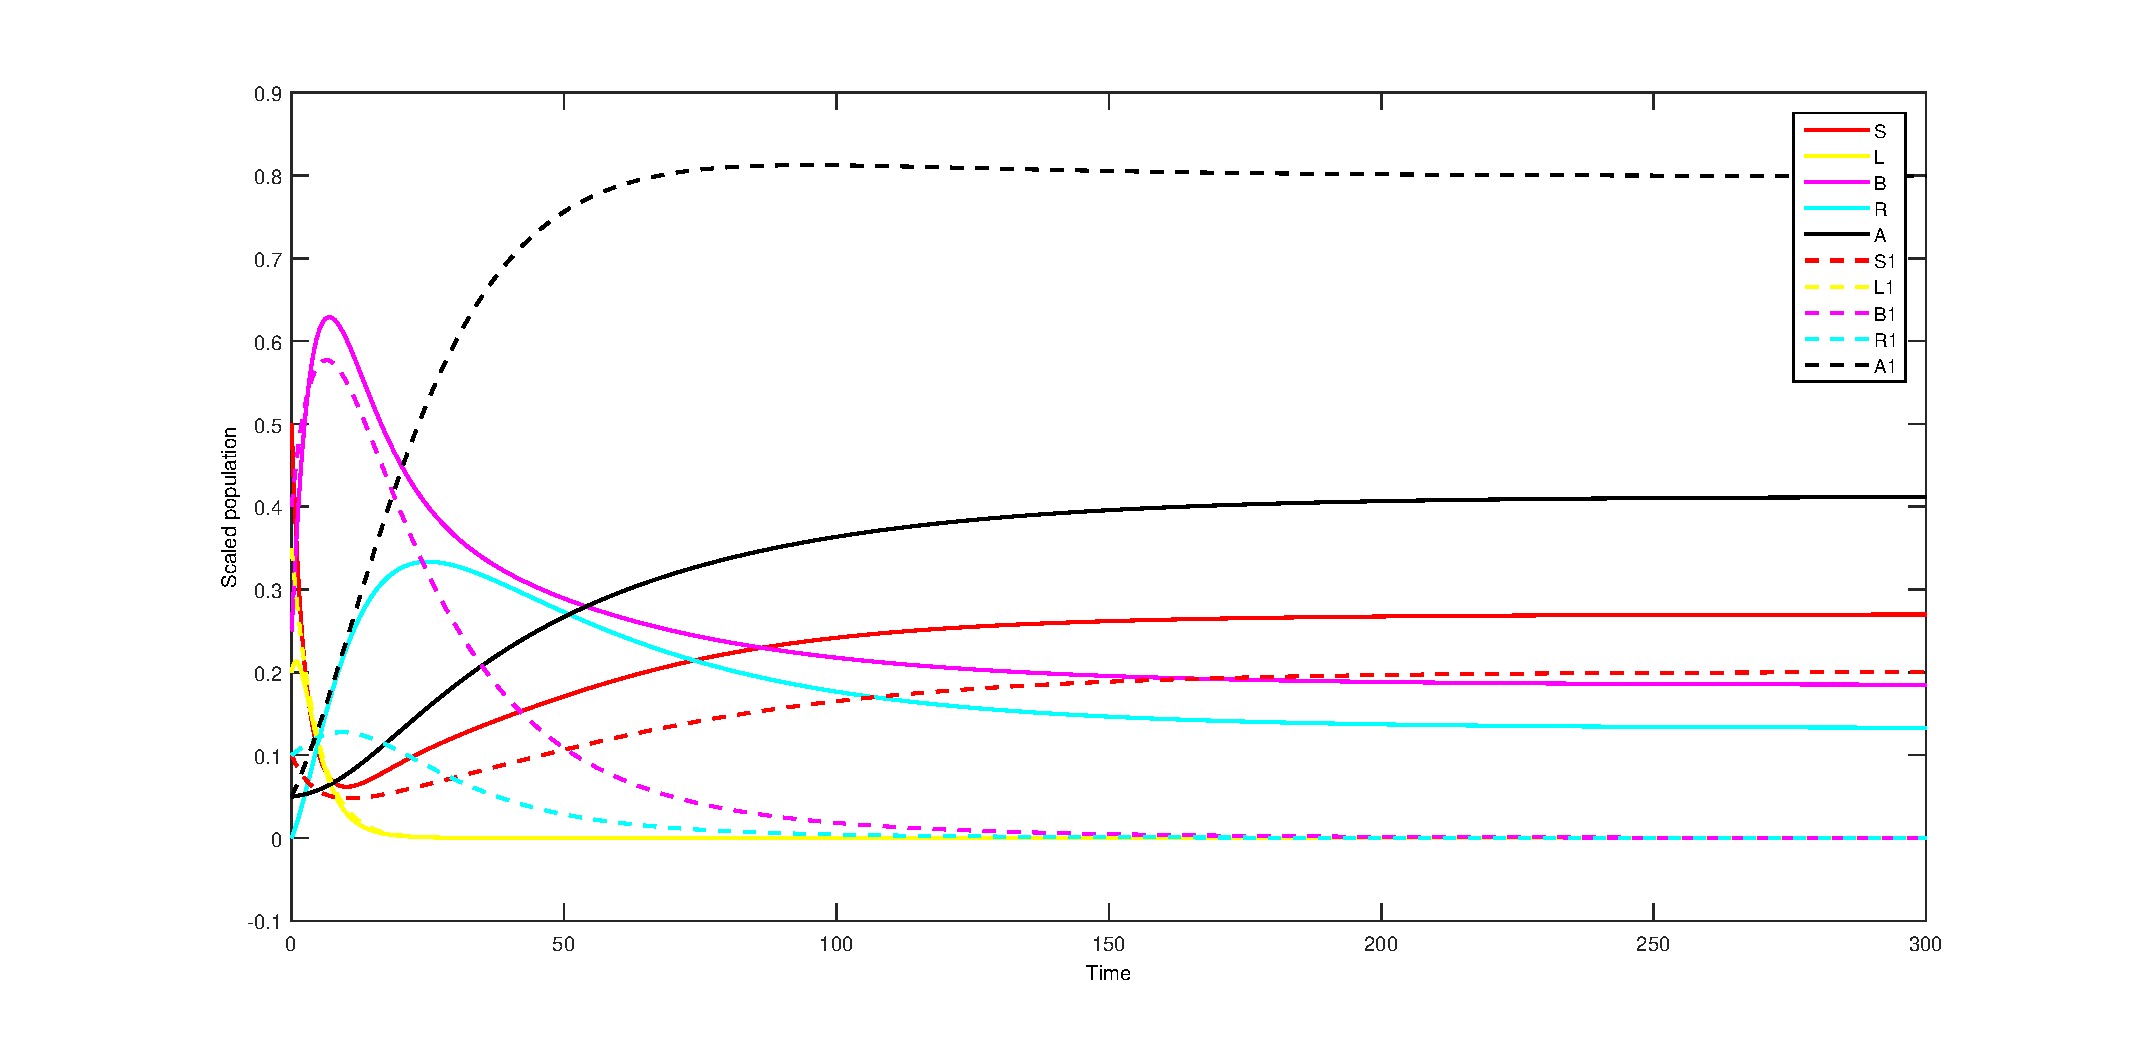
\includegraphics[width=0.8\columnwidth, clip=true]{1.eps}}
%\caption{Node Density vs. Time for different classes with Set 1}
%\end{figure}
%
%\begin{figure}
%\centering
%\subfigure[Node density of Set 2 with initial point(0.52 0.02 0.025 0.05 0.43 1 0 0 0 0)]{\label{fig:ff2}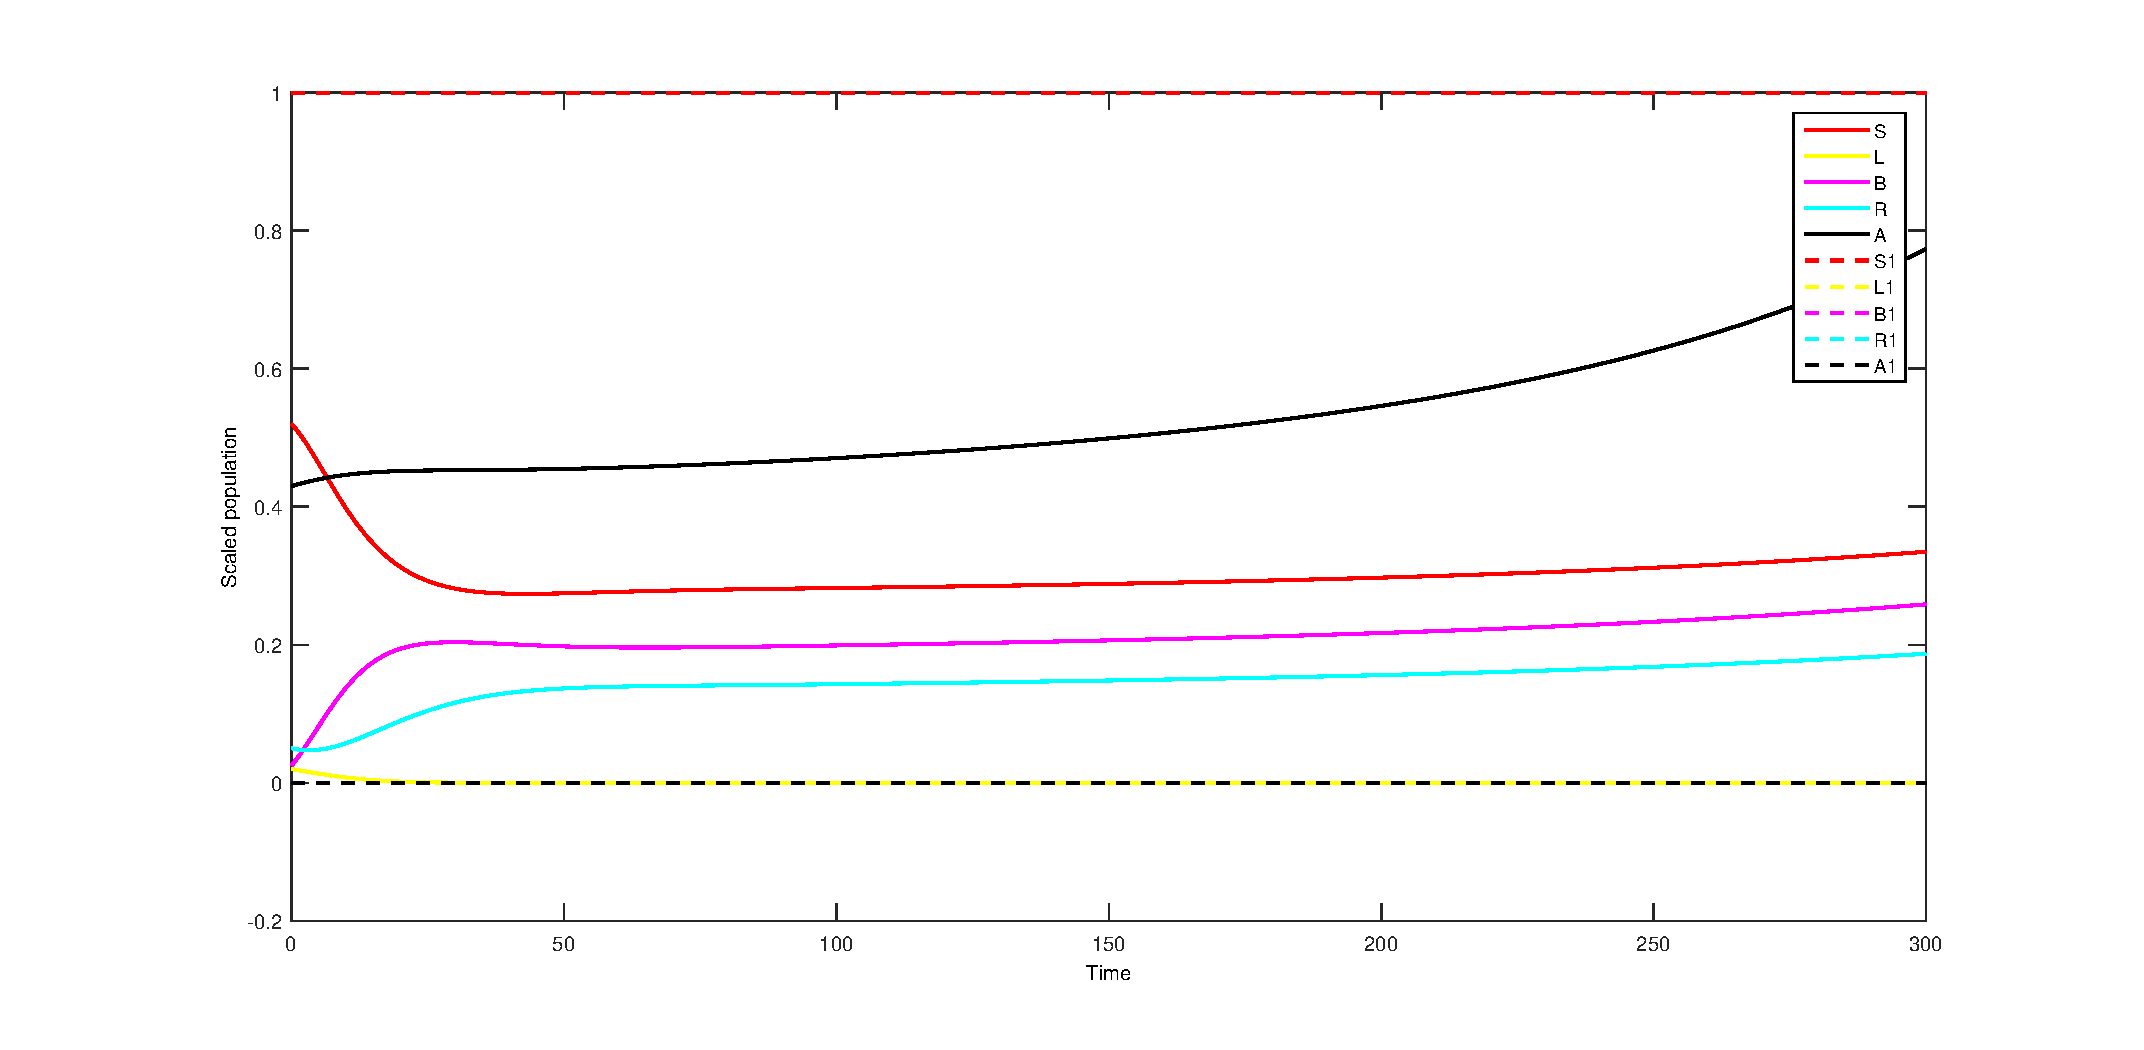
\includegraphics[width=0.8\columnwidth, clip=true]{2.eps}}
%\caption{Node Density vs. Time for different classes with Set 2}
%\end{figure}

\noindent Figure \ref{fig:ff3} is plotted with parameter set 2 and initial point (0.5, 0.2, 0.25, 0, 0.05, 0.1, 0.35, 0.4, 0.1, and 0.05).
Similarly, we can conclude that $ E_{1}, E_{2}, E_{3}$ and $E_{4}$ are the feasible steady states and $E_{4}$ is the stable steady state.

%\begin{figure}
%\centering
%\subfigure[Node density of Set 3 with initial point (0.5 0.2 0.25 0 0.05 0.1 0.35 0.4 0.1 0.05)]{\label{fig:ff3}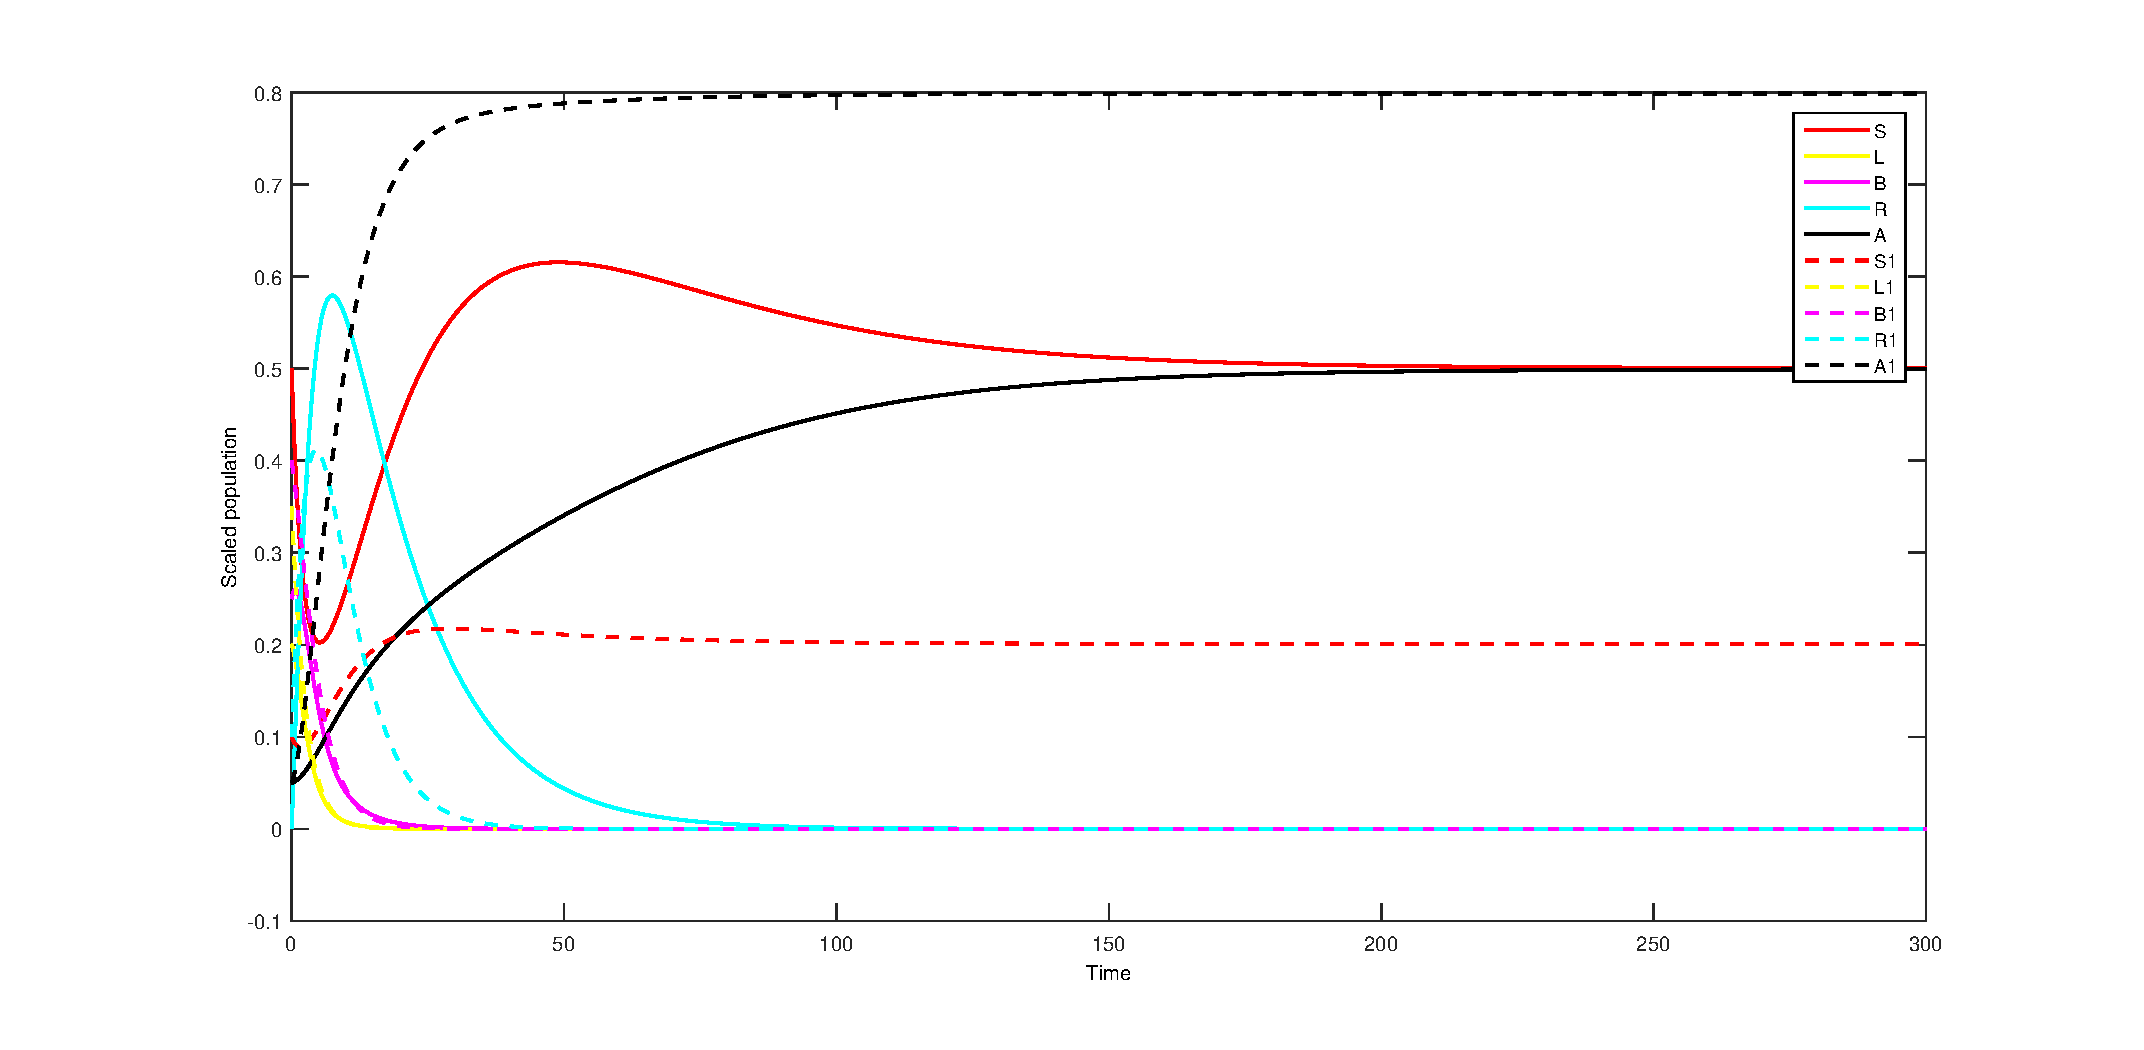
\includegraphics[width=0.8\columnwidth, clip=true]{3.eps}}
%\caption{Node Density vs. Time for different classes with Set 3}
%\end{figure}
%
%\newpage
%
%\begin{figure}
%\centering
%\subfigure[Node density of Set 4 with initial point (0.5 0.2 0.25 0 0.05 0.1 0.35 0.4 0.1 0.05)]{\label{fig:ff4}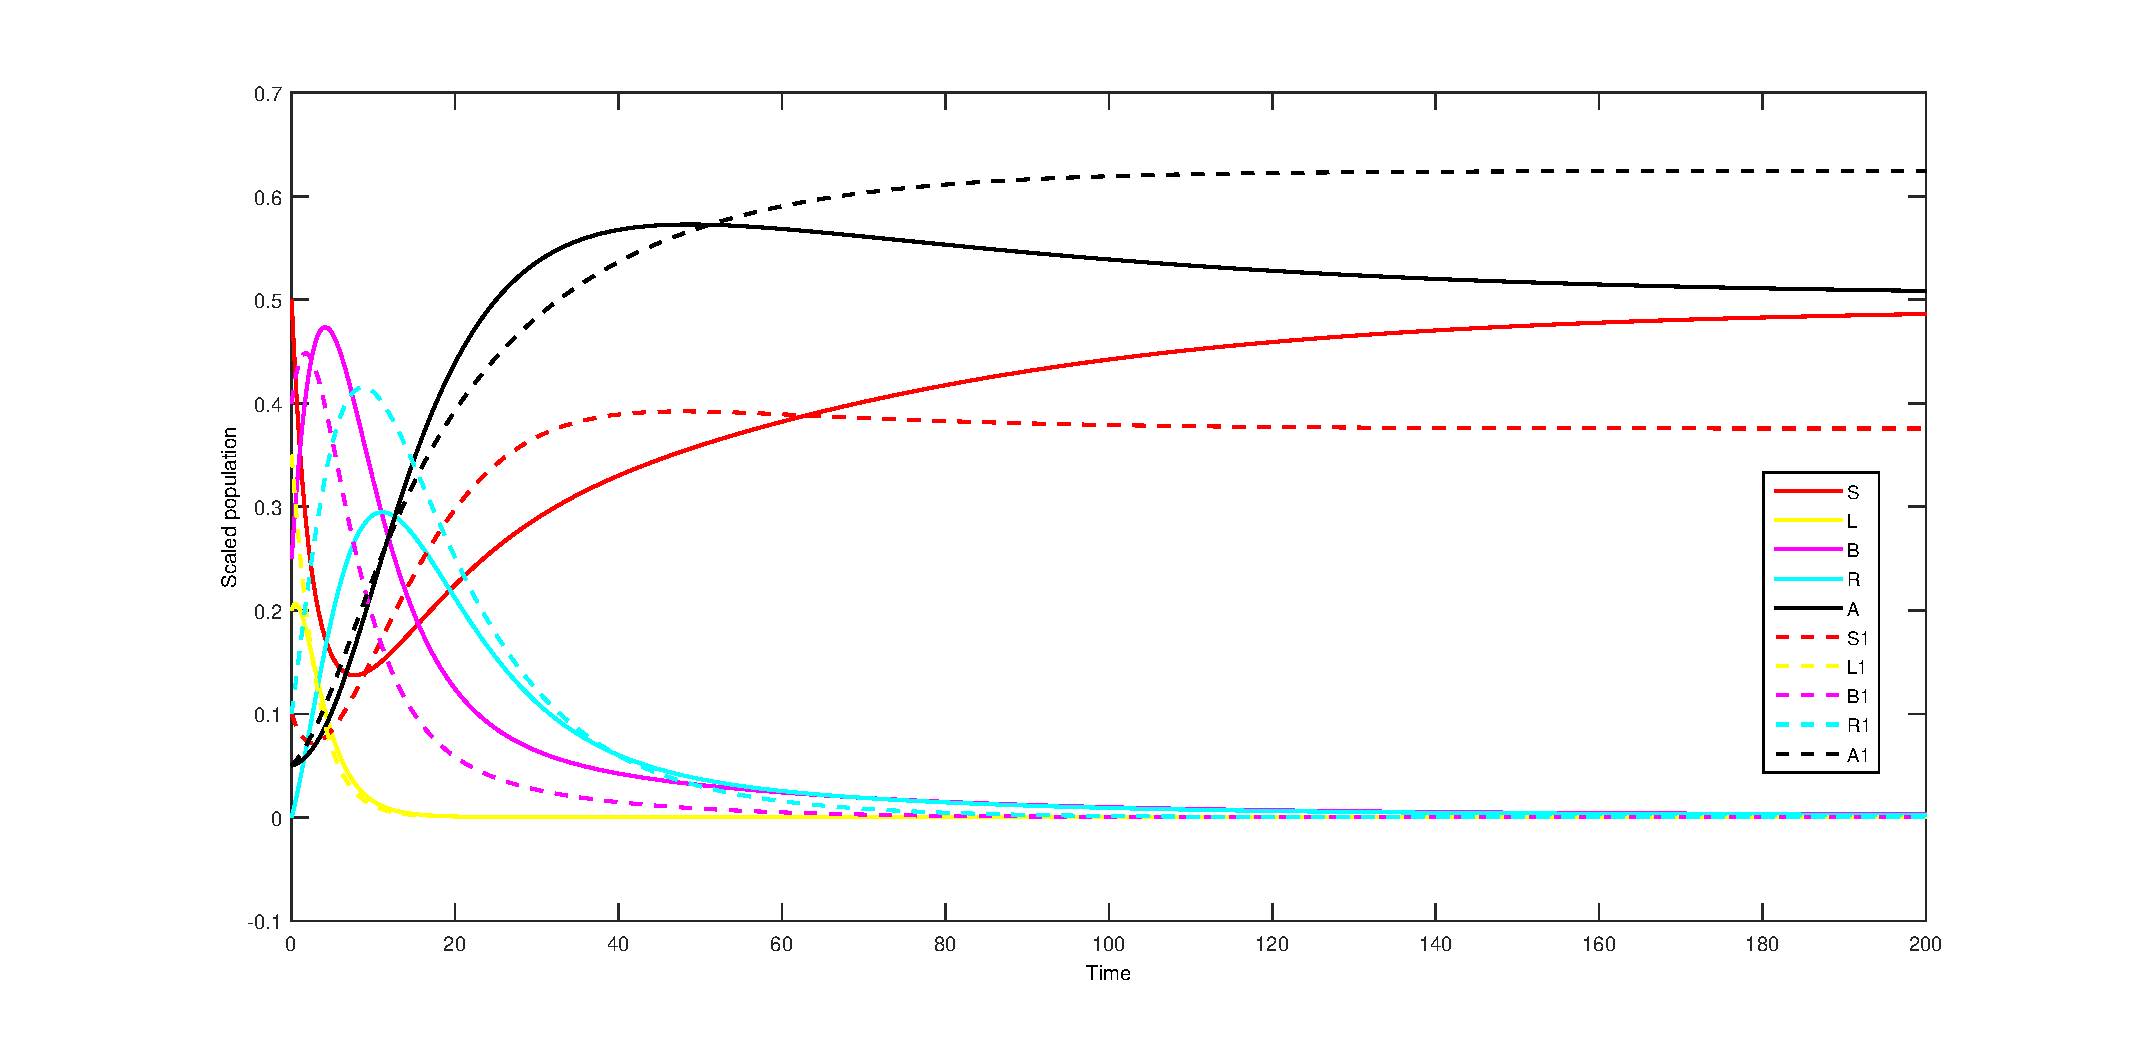
\includegraphics[width=0.8\columnwidth, clip=true]{4.eps}}
%\caption{Node Density vs. Time for different classes with Set 4}
%\end{figure}

\noindent Figure \ref{fig:ff4} is plotted with parameter set 3 and initial point (0.5, 0.2, 0.25, 0, 0.05, 0.1, 0.35, 0.4, 0.1 and 0.05). In this possible feasible states are $E_{3}$ and $ E_{4}$. Since one of the reproduction number is greater than 1, hence we can conclude that $E_{4}$ is the stable steady state.

\noindent Figure \ref{fig:ff5} is plotted with set 4 and initial point (0.2, 0, 0.25, 0.09, 0.46, 0.6, 0, 0, 0, and 0.4).
Similarly, we can conclude that $E_{3}, E_{4}, E_{9}$  and $E_{10}$ are the feasible steady states and $E_{10}$ is the stable steady state.
%\begin{figure}
%\centering
%\subfigure[Node density of Set 5 with initial point (0.2 0 0.25 0.09 0.46 0.6 0 0 0 0.4) ]{\label{fig:ff5}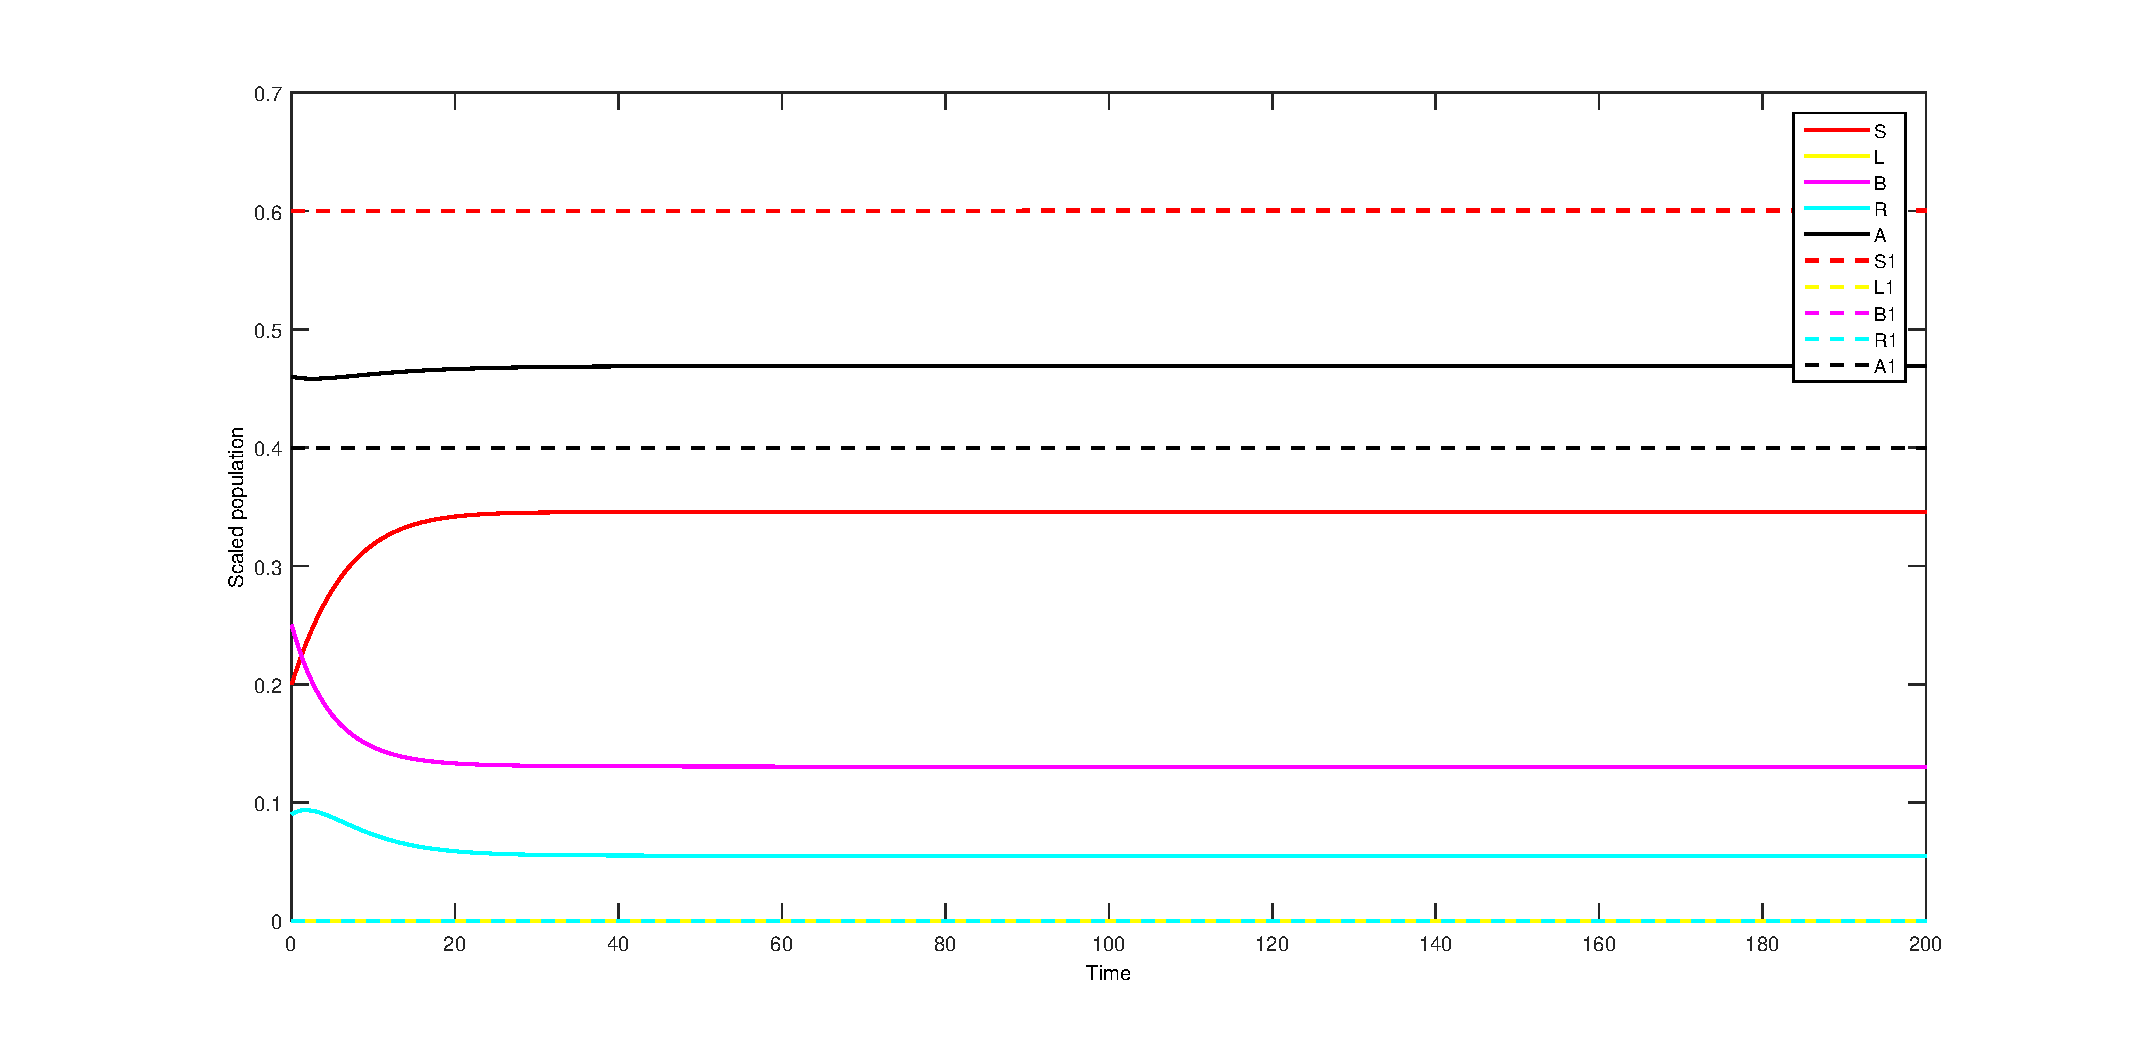
\includegraphics[width=0.8\columnwidth, clip=true]{5.eps}}
%\caption{Node Density vs. Time for different classes with Set 5}
%\end{figure}
%
%
%\begin{figure}
%\centering
%\subfigure[Node density of Set 6 with initial point (0.5 0.2 0.25 0 0.05 0.1 0.35 0.4 0.1 0.05) ]{\label{fig:ff6}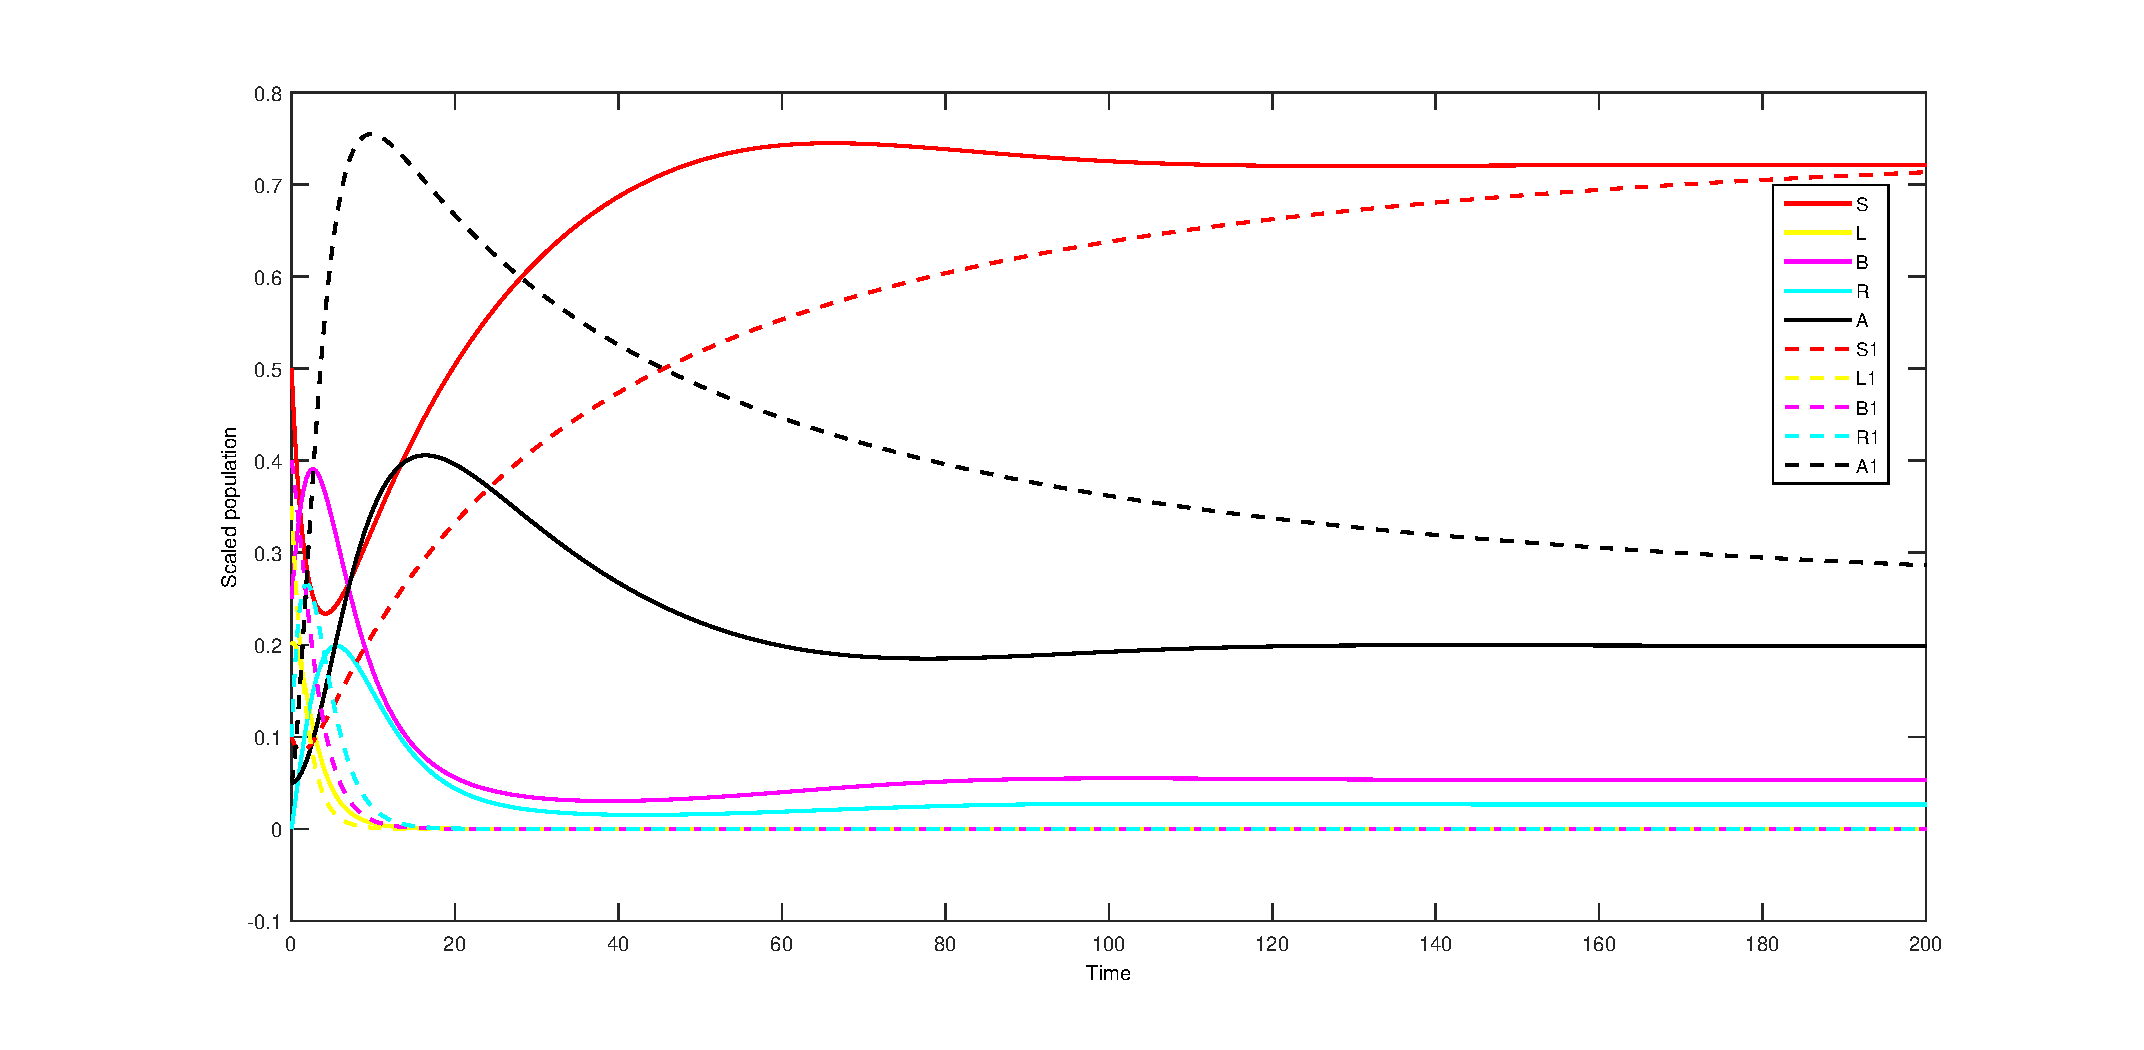
\includegraphics[width=0.8\columnwidth, clip=true]{7.eps}}
%\caption{Node Density vs. Time for different classes with Set 6}
%\end{figure}

\noindent Figure \ref{fig:ff6} is plotted with parameter set 5 and initial point (0.5, 0.2, 0.25, 0, 0.05, 0.1, 0.35, 0.4, 0.1 and 0.05). In this observed feasible states are $ E_{9}$ and  $E_{10}$. From the figure it is clear that $E_{10}$ is the stable steady state.

\noindent Figures \ref{fig:ff7} and \ref{fig:ff8} are plotted with different initial points for parameter set 6 and the observed feasible states are $ E_{3}$ and  $E_{4}$. For the initial point (0.5 0.02 0.03 0 0.45 1 0 0 0 0), $E_{3}$ is the observed stable steady state and $E_{4}$ is the observed stable steady state for the initial point (0.5 0.2 0.25 0 0.05 0.1 0.35 0.4 0.1 0.05).

\newpage
\begin{figure}[h!]
\centering
  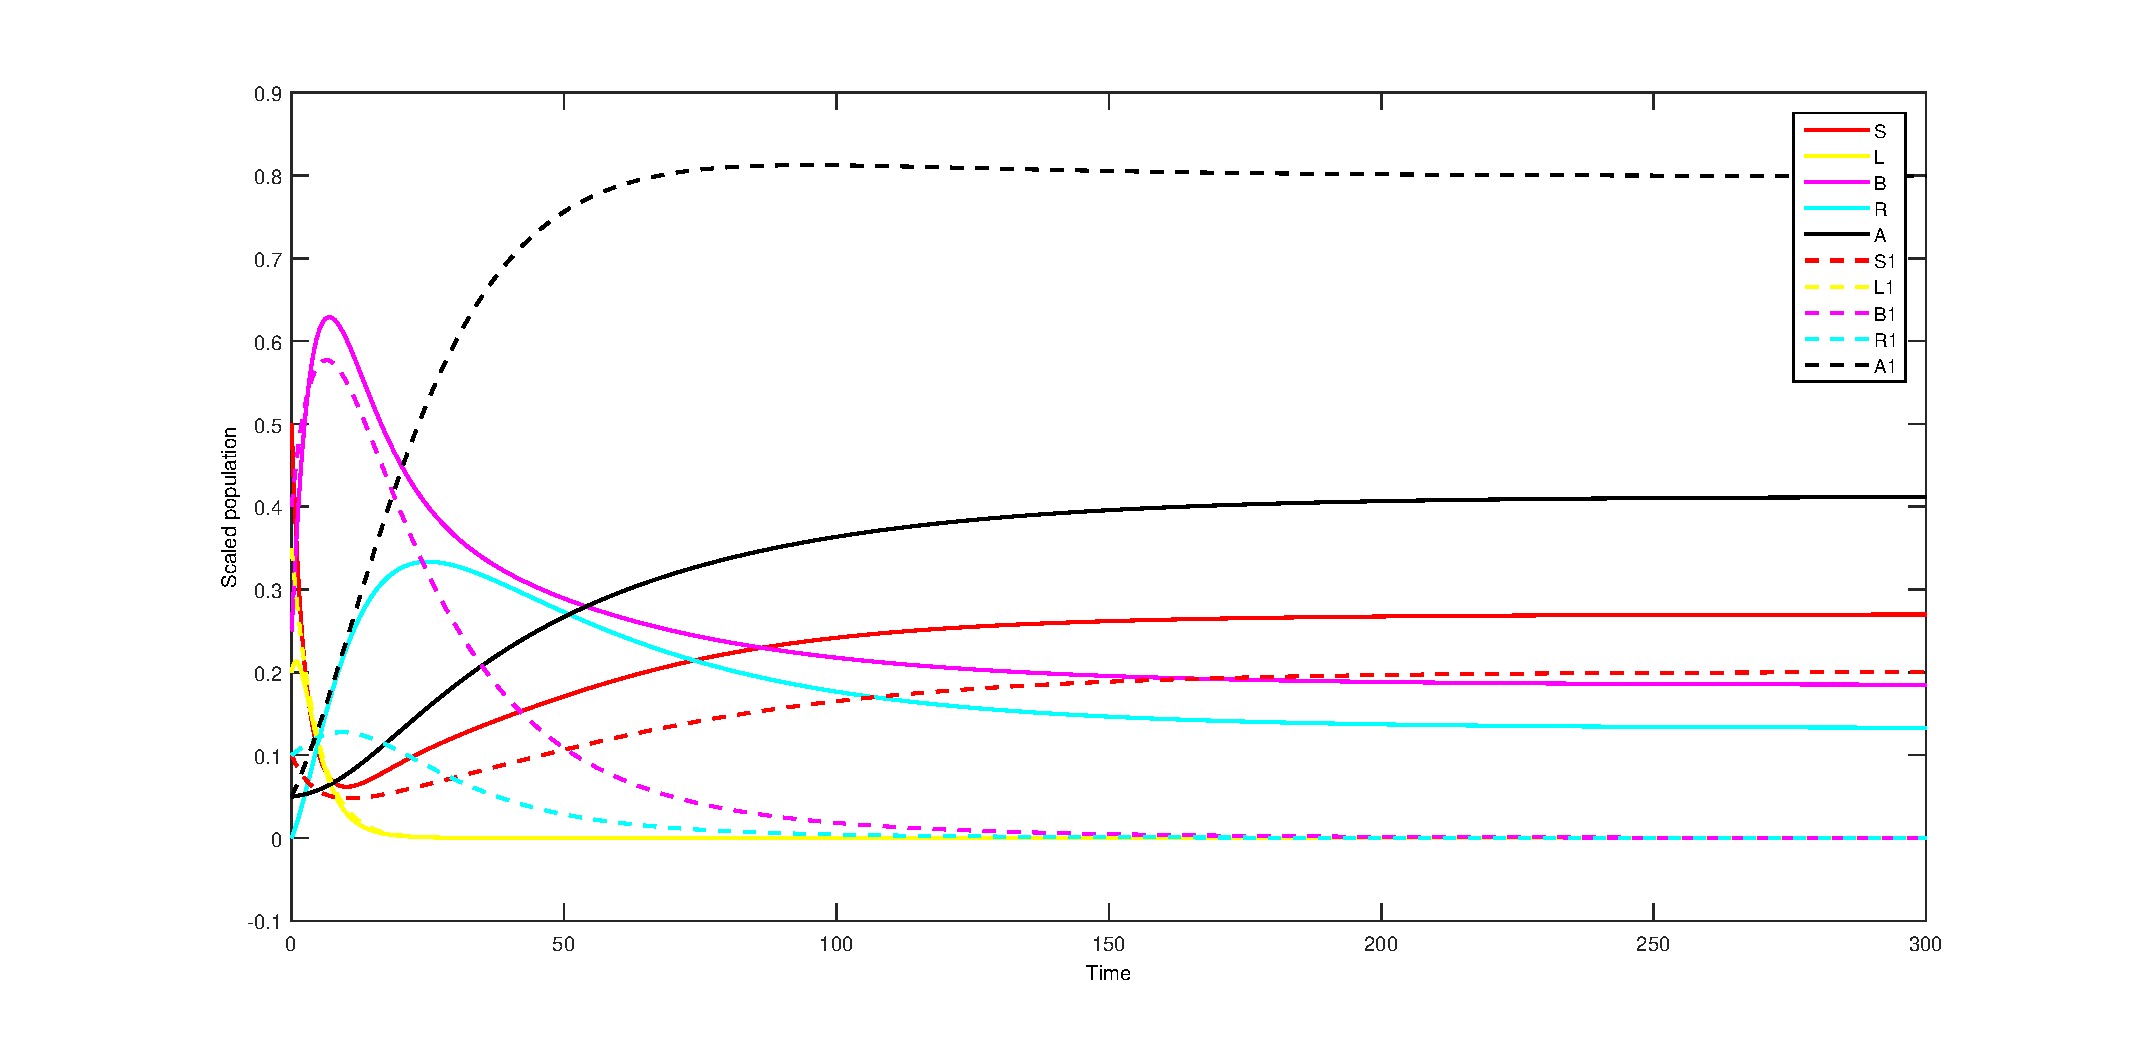
\includegraphics[width=7.0in]{1.eps}\\
  \caption{Node Density vs. Time for set 1 initial point(0.5 0.2 0.25 0 0.05 0.1 0.35 0.4 0.1 0.05)}\label{fig:ff0}
\end{figure}

\begin{figure}[h!]
\centering
  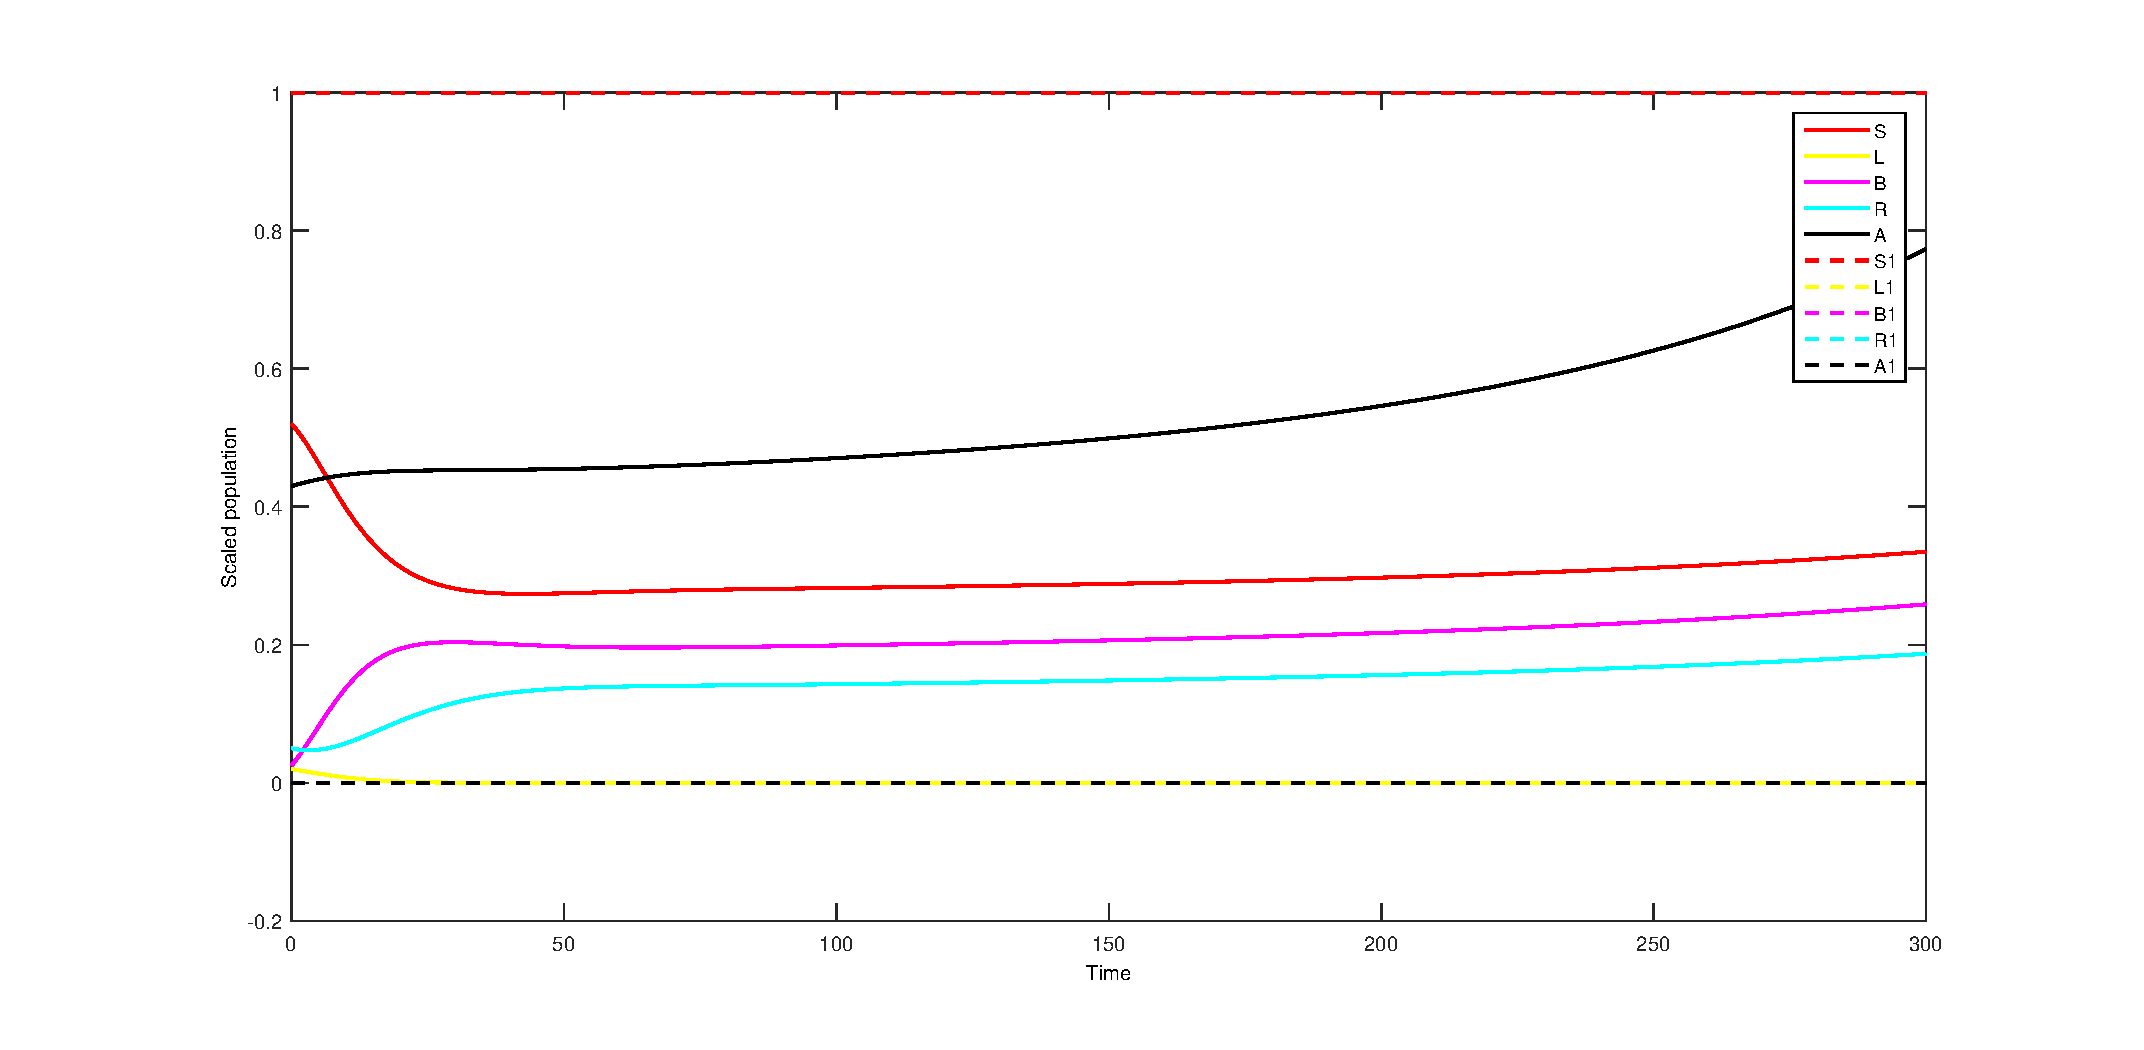
\includegraphics[width=7.0in]{2.eps}\\
  \caption{Node Density vs. Time for set 1 initial point(0.52 0.02 0.025 0.05 0.43 1 0 0 0 0)}\label{fig:ff2}
\end{figure}

\newpage
\begin{figure}[h!]
\centering
  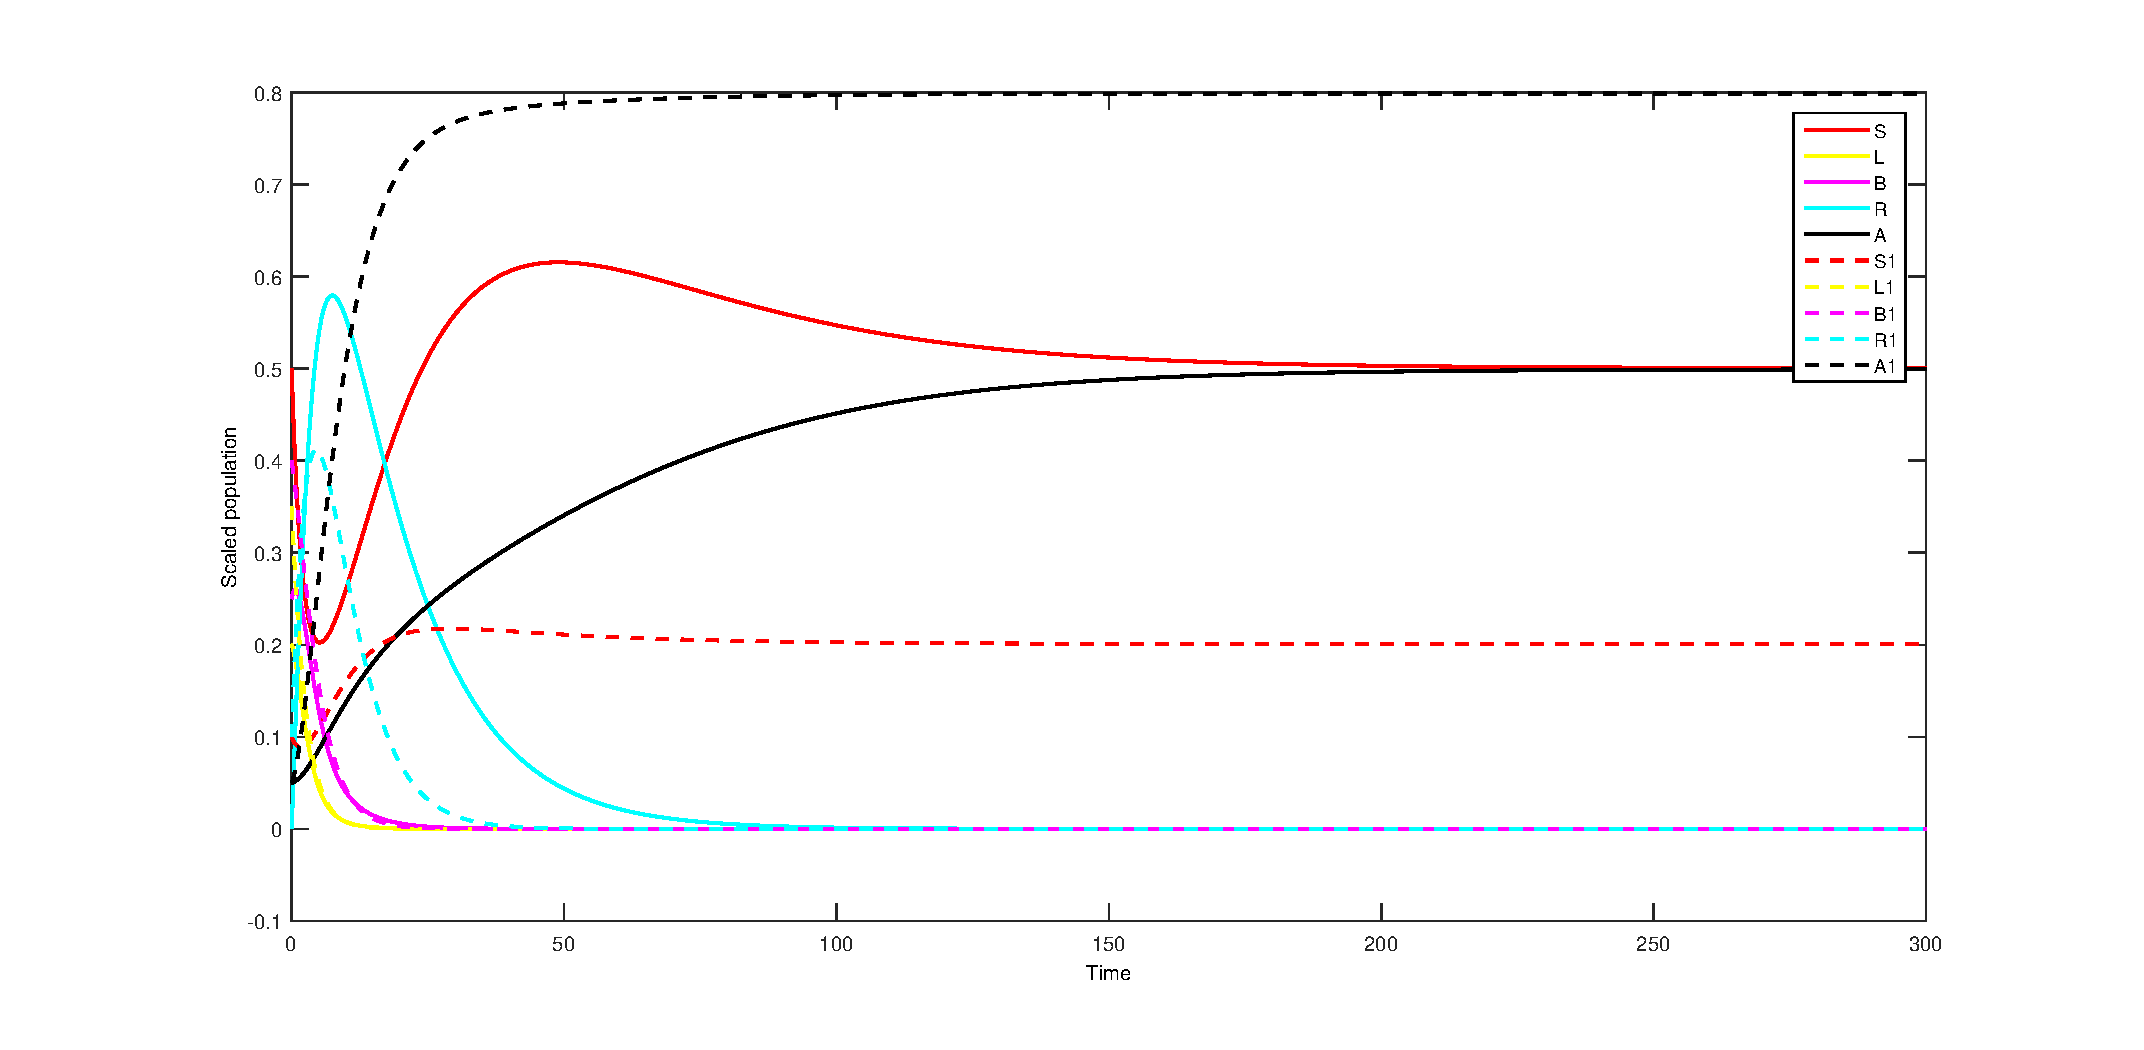
\includegraphics[width=7.0in]{3.eps}\\
  \caption{Node Density vs. Time for set 2 initial point(0.5 0.2 0.25 0 0.05 0.1 0.35 0.4 0.1 0.05)}\label{fig:ff3}
\end{figure}

\begin{figure}[h!]
\centering
  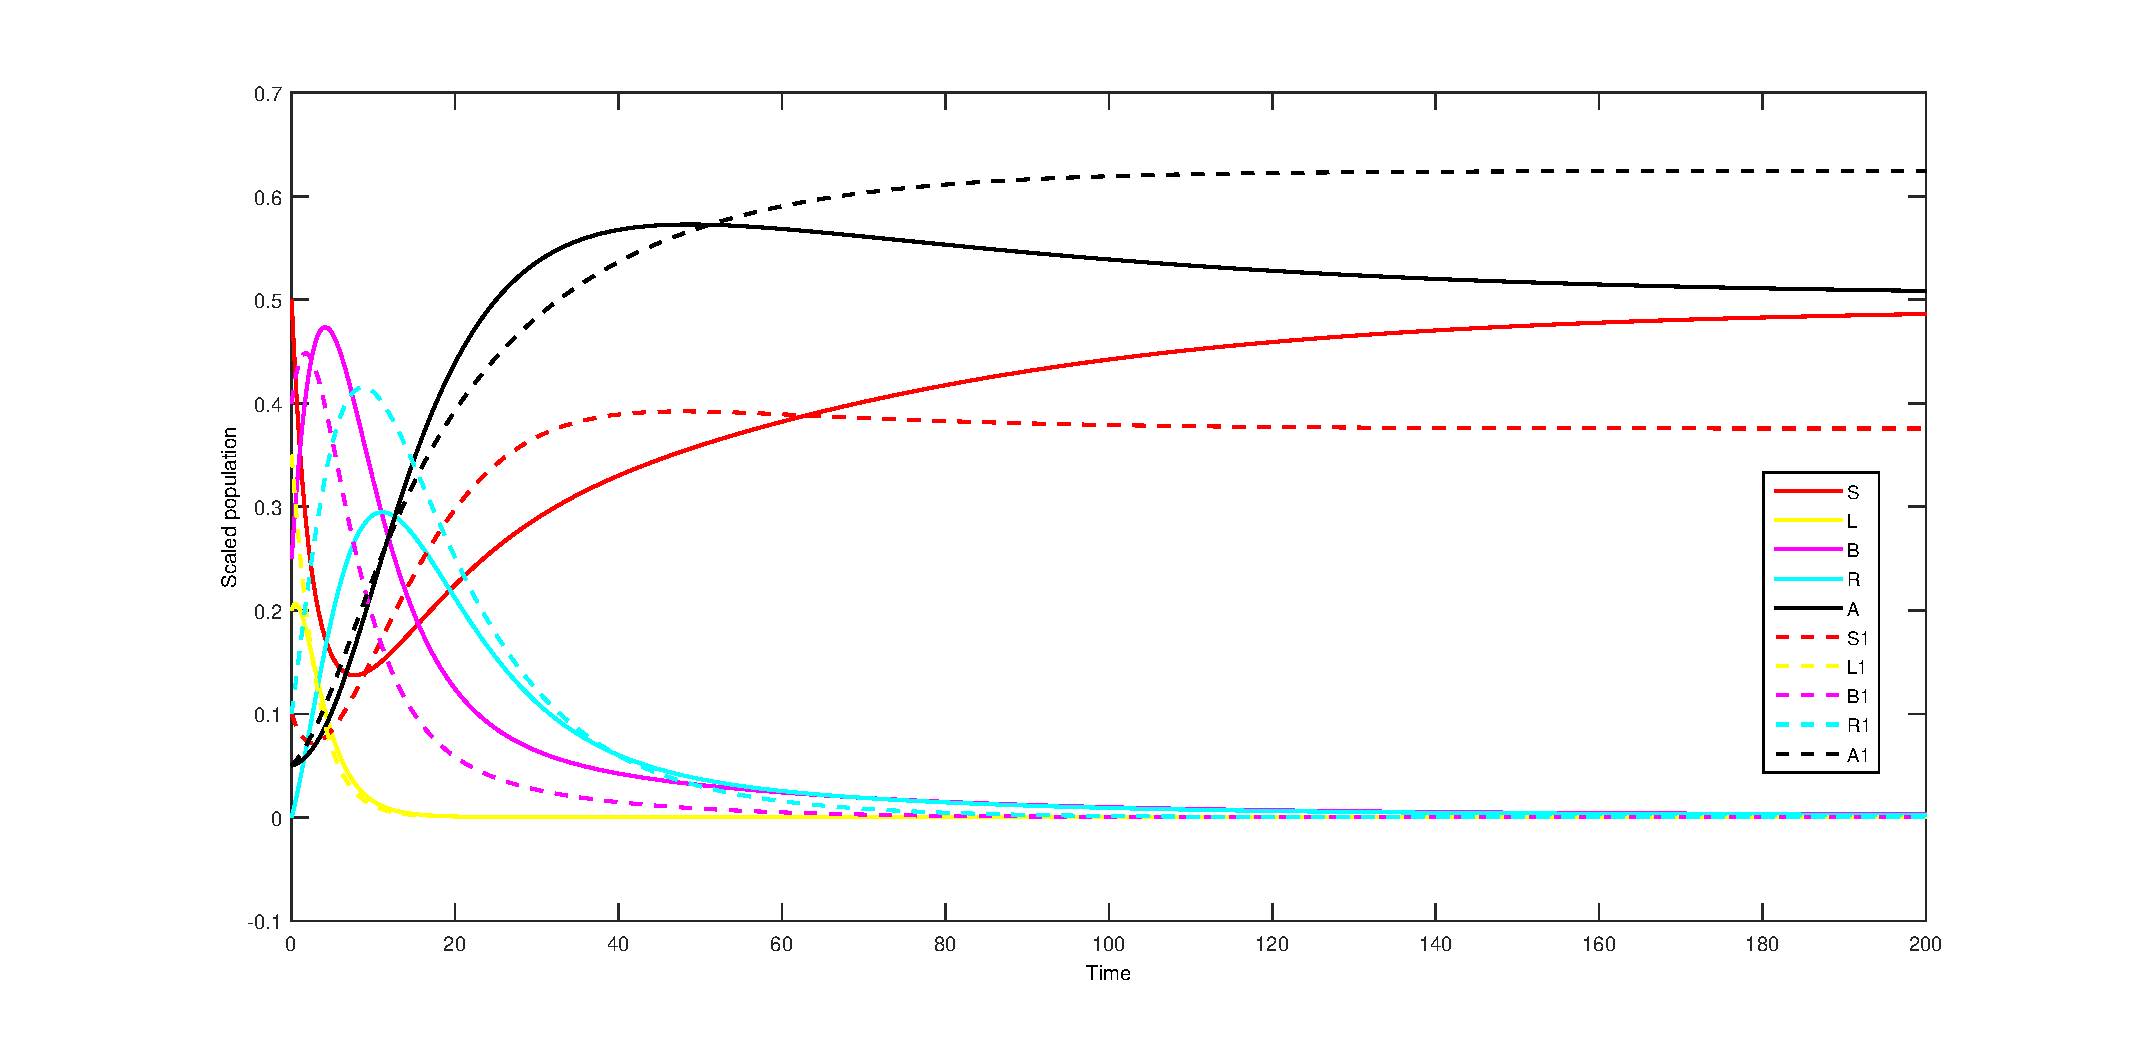
\includegraphics[width=7.0in]{4.eps}\\
  \caption{Node Density vs. Time for set 3 initial point(0.5 0.2 0.25 0 0.05 0.1 0.35 0.4 0.1 0.05)}\label{fig:ff4}
\end{figure}

\newpage
\begin{figure}[h!]
\centering
  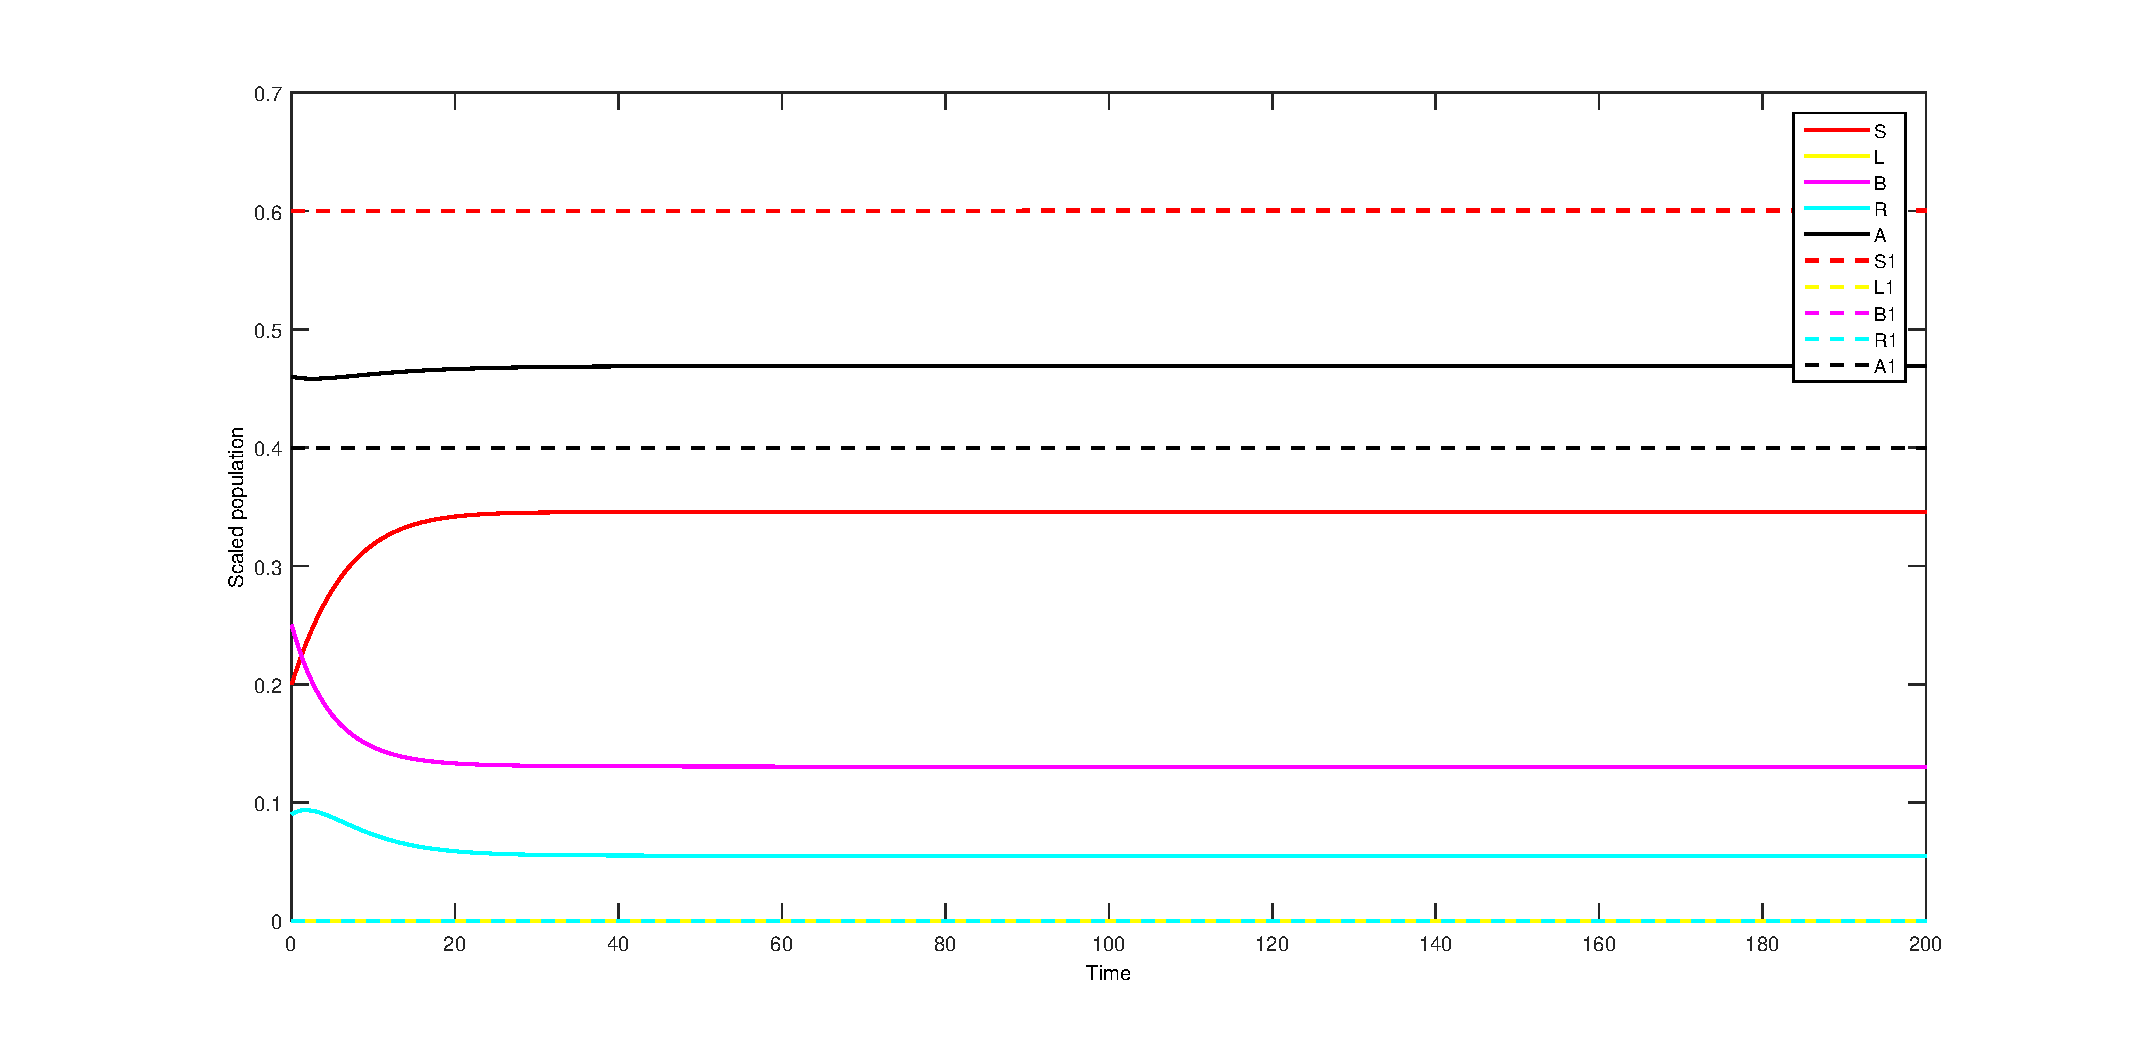
\includegraphics[width=7.0in]{5.eps}\\
  \caption{Node Density vs. Time for set 4 initial point(0.2 0 0.25 0.09 0.46 0.6 0 0 0 0.4)}\label{fig:ff5}
\end{figure}

\begin{figure}[h!]
\centering
  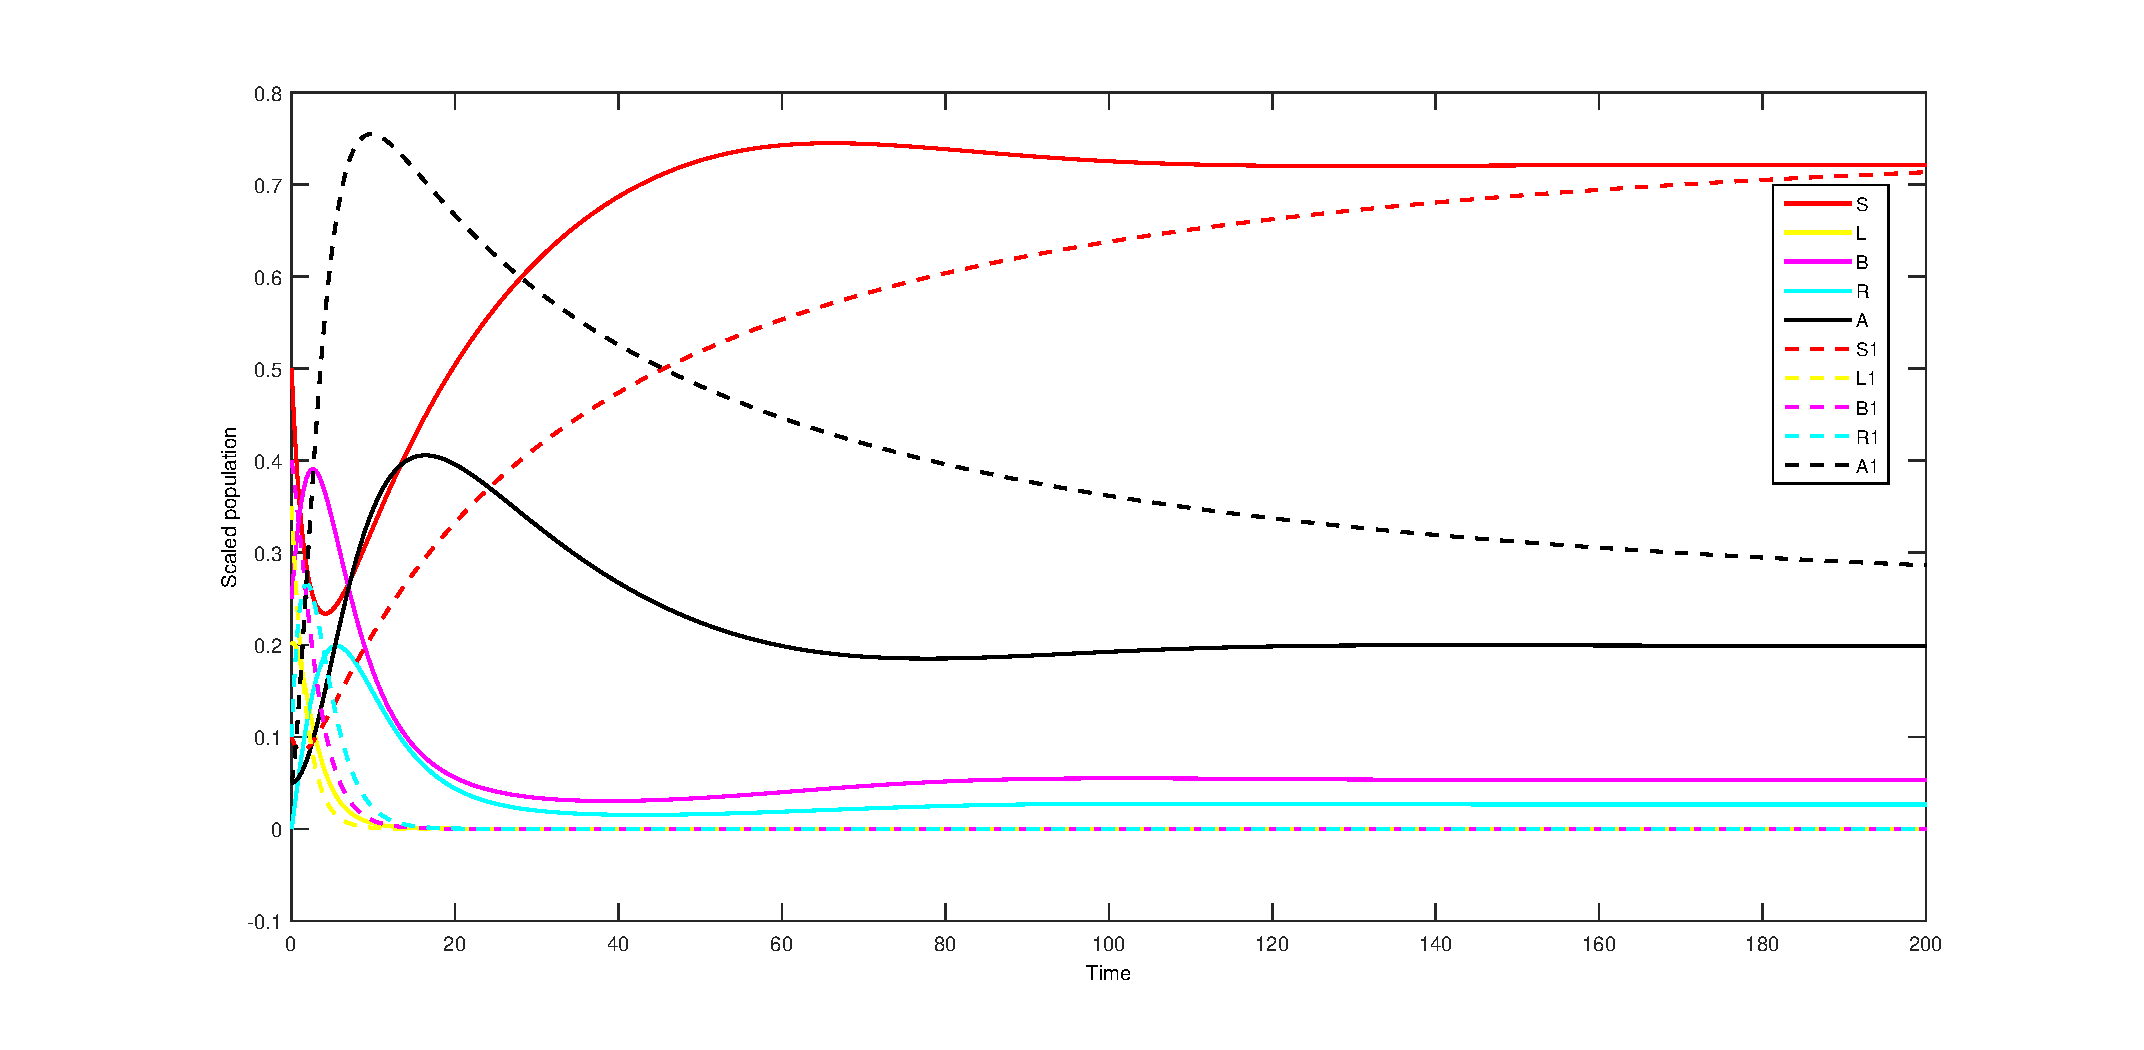
\includegraphics[width=7.0in]{7.eps}\\
  \caption{Node Density vs. Time for set 5 initial point(0.5 0.2 0.25 0 0.05 0.1 0.35 0.4 0.1 0.05)}\label{fig:ff6}
\end{figure}

\newpage
\begin{figure}[h!]
\centering
  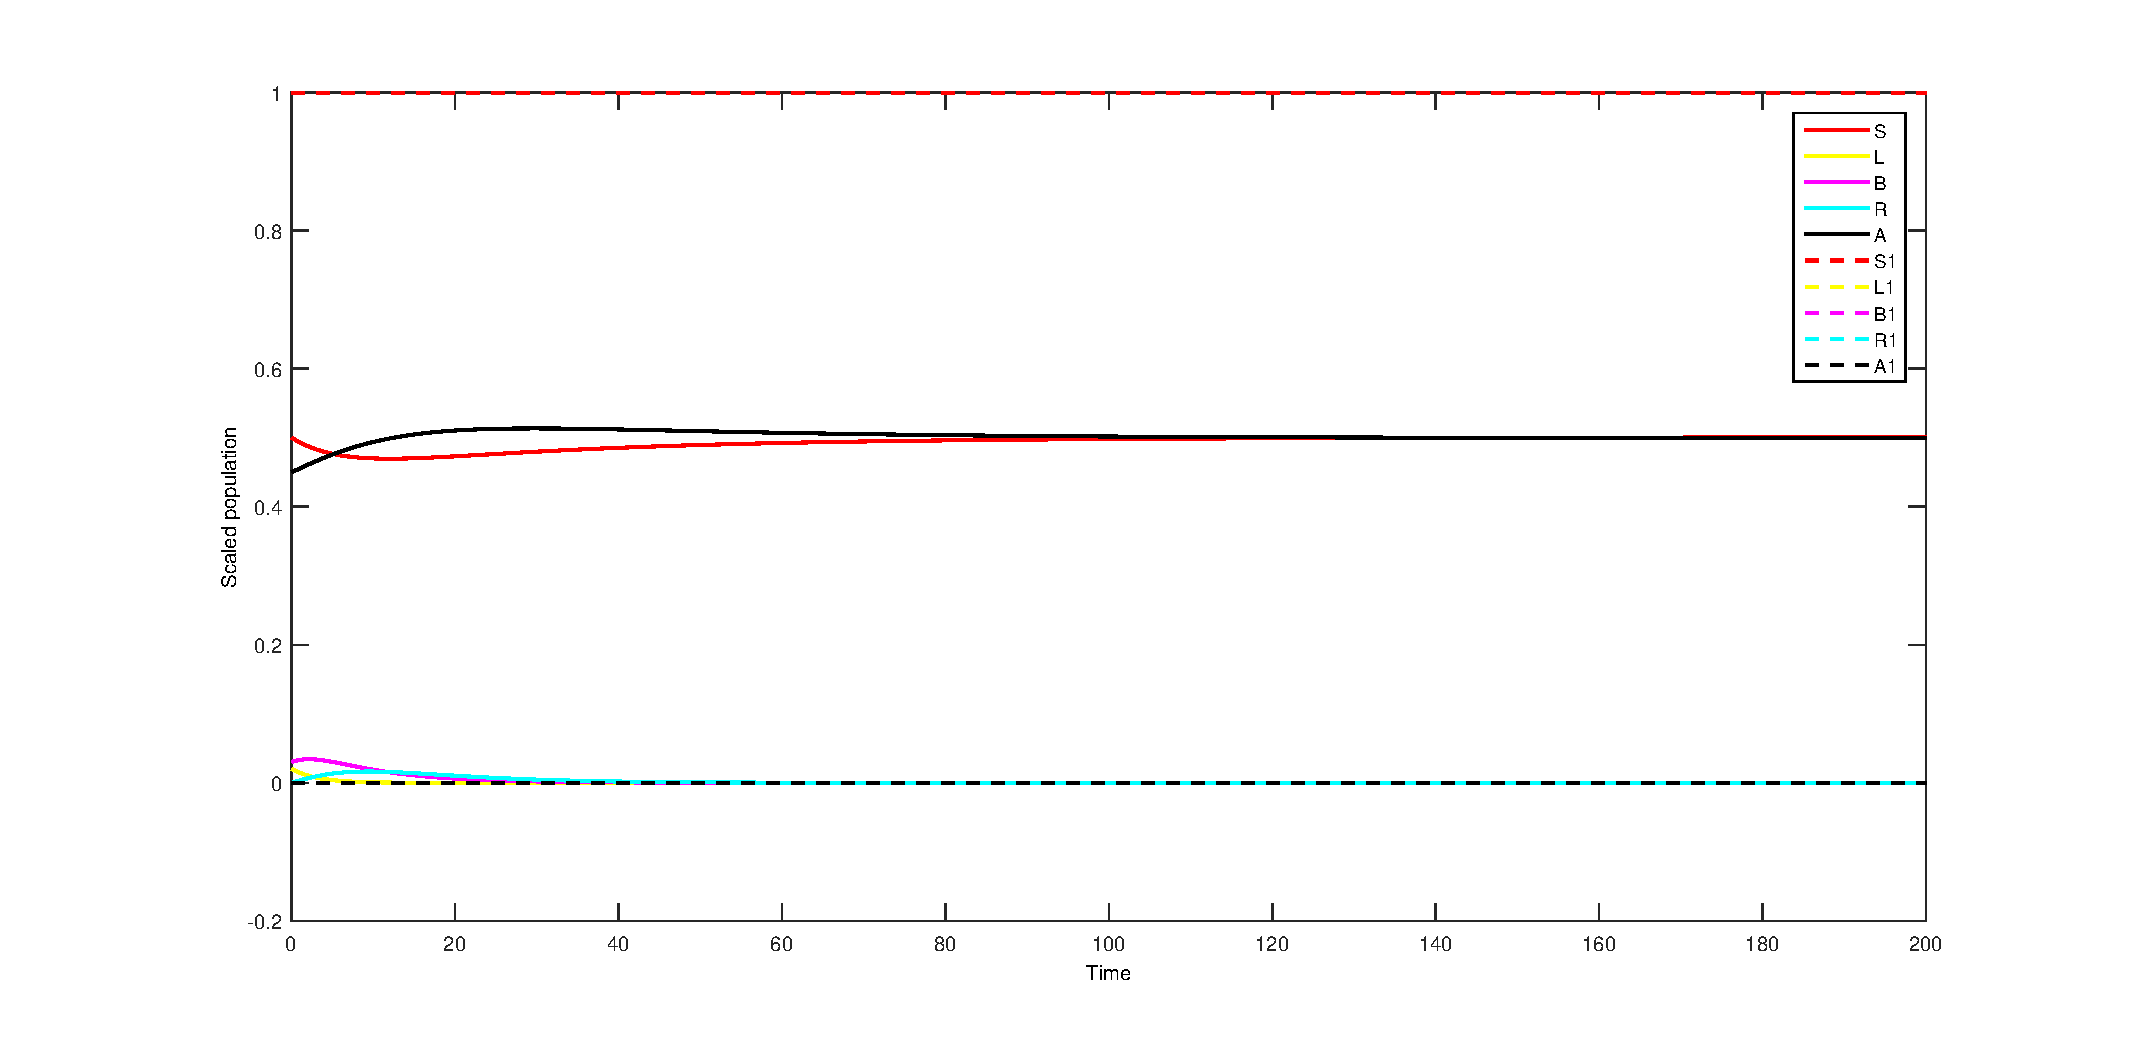
\includegraphics[width=7.0in]{8.eps}\\
  \caption{Node Density vs. Time for set 6 initial point(0.5 0.02 0.03 0 0.45 1 0 0 0 0)}\label{fig:ff7}
\end{figure}
\begin{figure}[h!]
\centering
  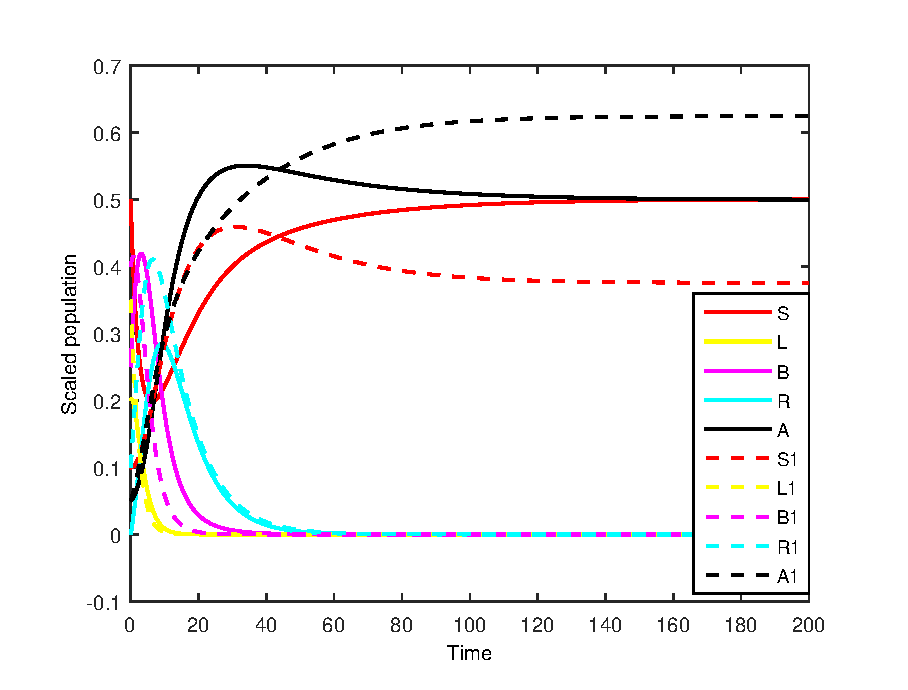
\includegraphics[width=7.0in,height=3.3in]{9.eps}\\
  \caption{Node Density vs. Time for set 6 initial point(0.5 0.2 0.25 0 0.05 0.1 0.35 0.4 0.1 0.05)}\label{fig:ff8}
\end{figure}

\newpage
\section{Estimation of Firewall Security Coefficient}
The firewall is the central security of a network. The objective of the firewall is to create rules and policies which allows only particular connections.
\subsection{Order of rule enforcement}
The firewall keeps track of every connection and enforces the rule base sequentially. The firewall monitors every connection and compares that connection for the consistency with service, data and destination. If the connection is valid then firewall applies that rule otherwise, it checks for the next matching rule in the Rule base.
%\begin{figure}
%\centering
%\subfigure[Node density of Set 1 with initial point (1, 1, 1, 1, 1, 1) ]{\label{fig:a2}\includegraphics[width=60mm,height=45mm]{Set1.png}}
%\label{graph_SLBRA}
%\end{figure}
\subsection{Firewall rule priority}
Since we can define firewall rules that have apparent conflicts, it is important to understand the sequence in which the rules are executed.
\subsection{Authenticated bypass}
 These rules allow matched network traffic otherwise it would be blocked. A separate connection security rule would be used to authenticate the network traffic. These rules are used to allow access to any computer to an authorized troubleshooting device and network administrator.
%\end{subsection}
\subsection{Block connection}
       These rules restrict all matched incoming network traffic.
%\end{subsection}
\subsection{Allow connection}
        These defined rules allow matched incoming network traffic. Because the general criteria is to restrict distrustful incoming network traffic, we must define an allow rule to help any network program or service that must be able to accept incoming connections.\\
      The coefficient of firewall security, m should depend on the types of files(data) under consideration, defined firewall security rules in the firewall rule base and the reliability and efficiency of the firewall. We define a way for
          measuring the value m of firewall security as:
          $$m=-{\log_e (a+b-ab)},$$
          where, 'b' measures the response of the files to the defined security rules.
For our work we can add certain rules by monitoring the behavior of attacker class. When the files will be received in targeted class, they will be checked according to the rules defined in the firewall rule base. If they response correctly to all these rules then 'b'=0 and if they don't match any of the rules then 'b'=1 and it is supposed that the malware propagation rate can be reduced by proportion 'a', when each received files abide the defined security rules.
\newpage
\begin{figure}[h!]
  % Requires \usepackage{graphicx}
  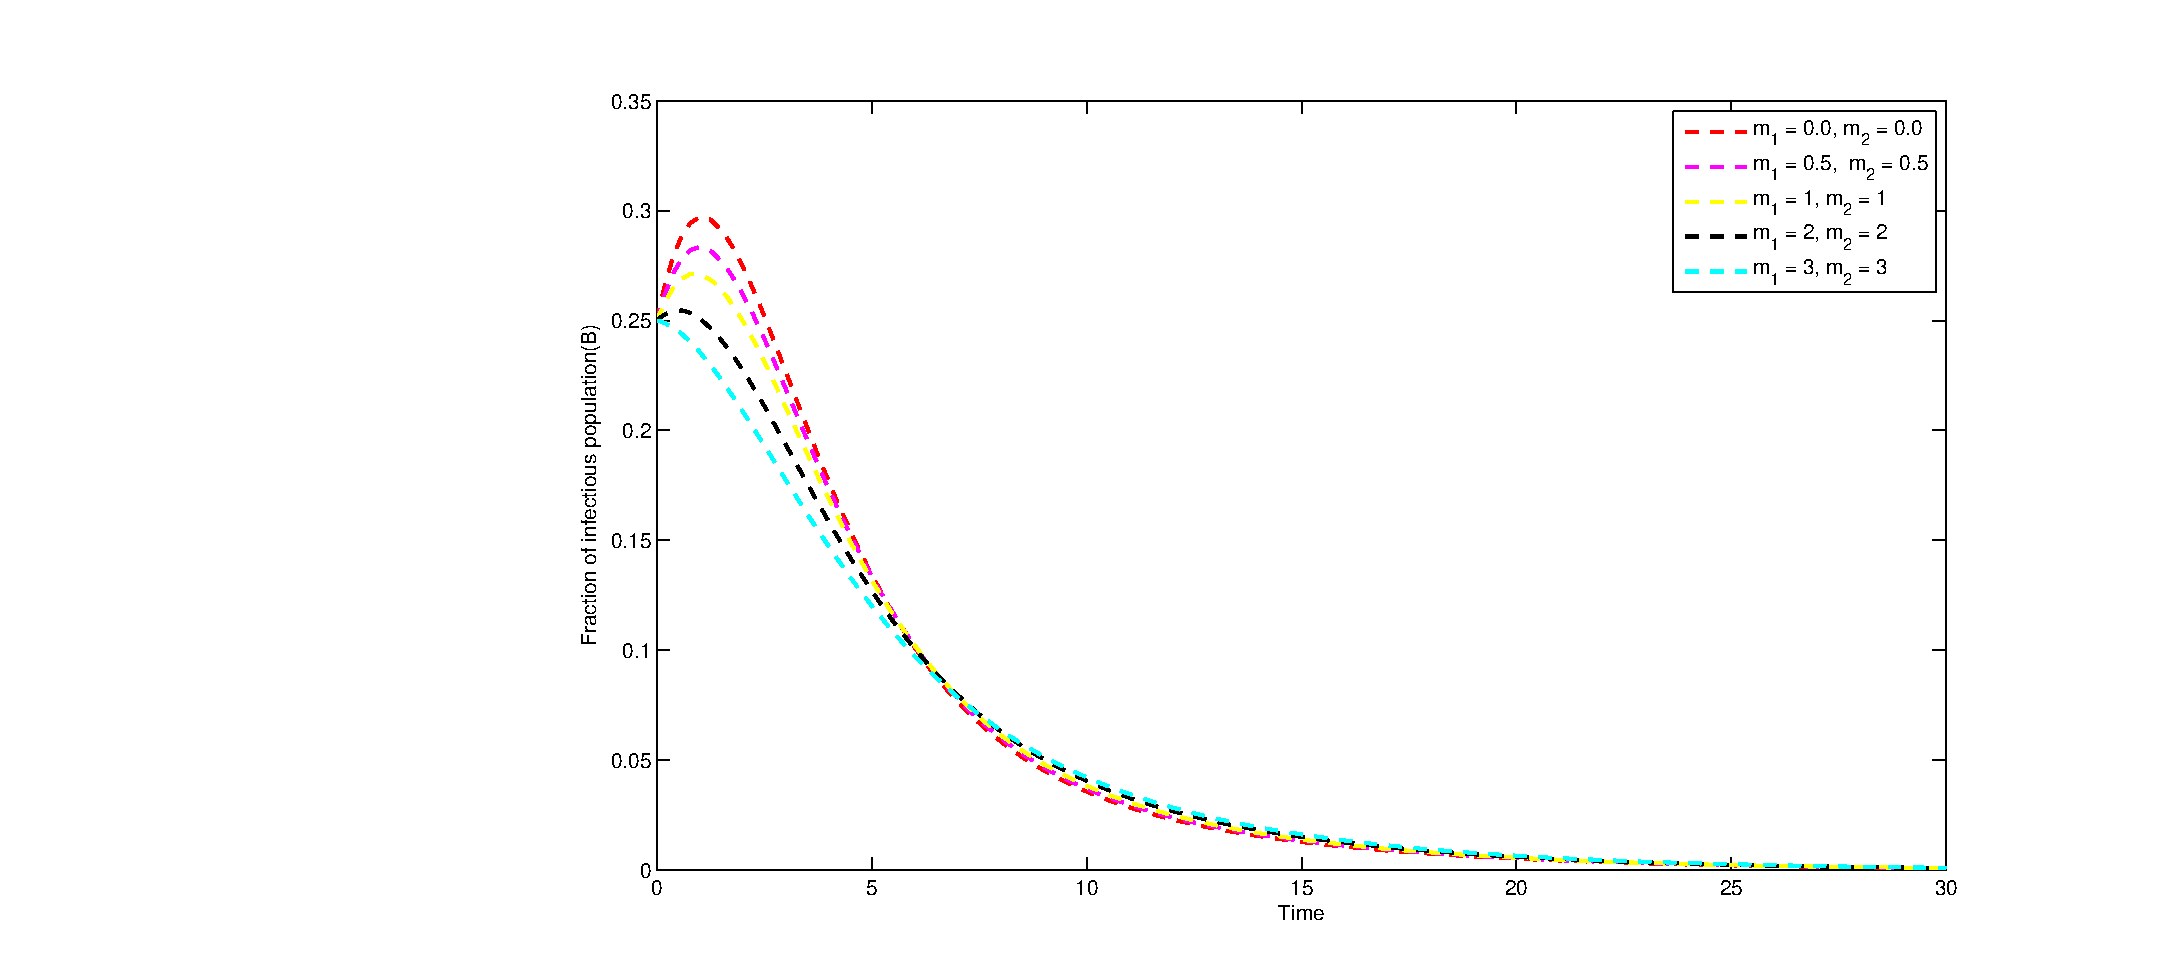
\includegraphics[width=7.5in]{mB1.eps}\\
  \caption{Effect of m on B when $R_0<1$}\label{fig:a2}
\end{figure}
%\end{center}
\begin{flushleft}
\begin{figure}[h!]
\centering
  % Requires \usepackage{graphicx}
  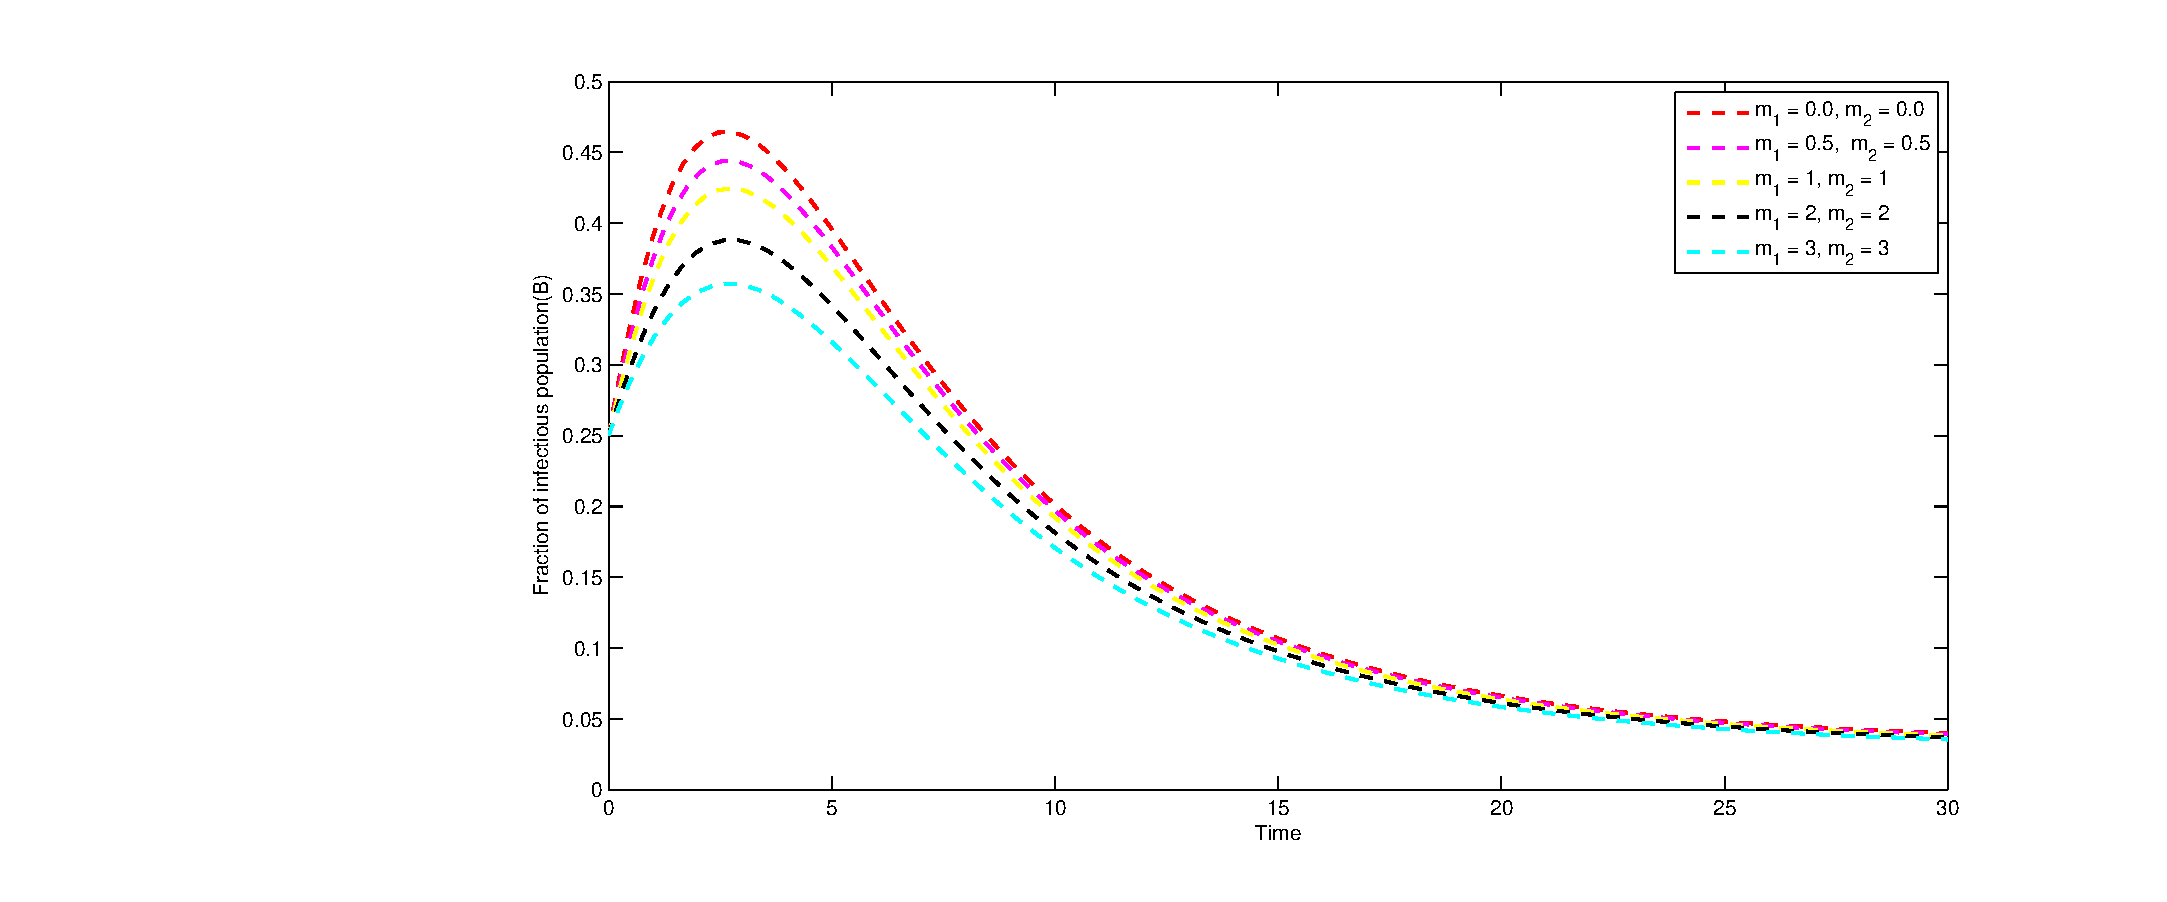
\includegraphics[width=7.5in]{mB2.eps}\\
  \caption{Effect of m on B when $R_0>1$}\label{fig:b2}
\end{figure}
\end{flushleft}

\newpage
\begin{flushleft}
\begin{figure}[h!]
\centering
  % Requires \usepackage{graphicx}
  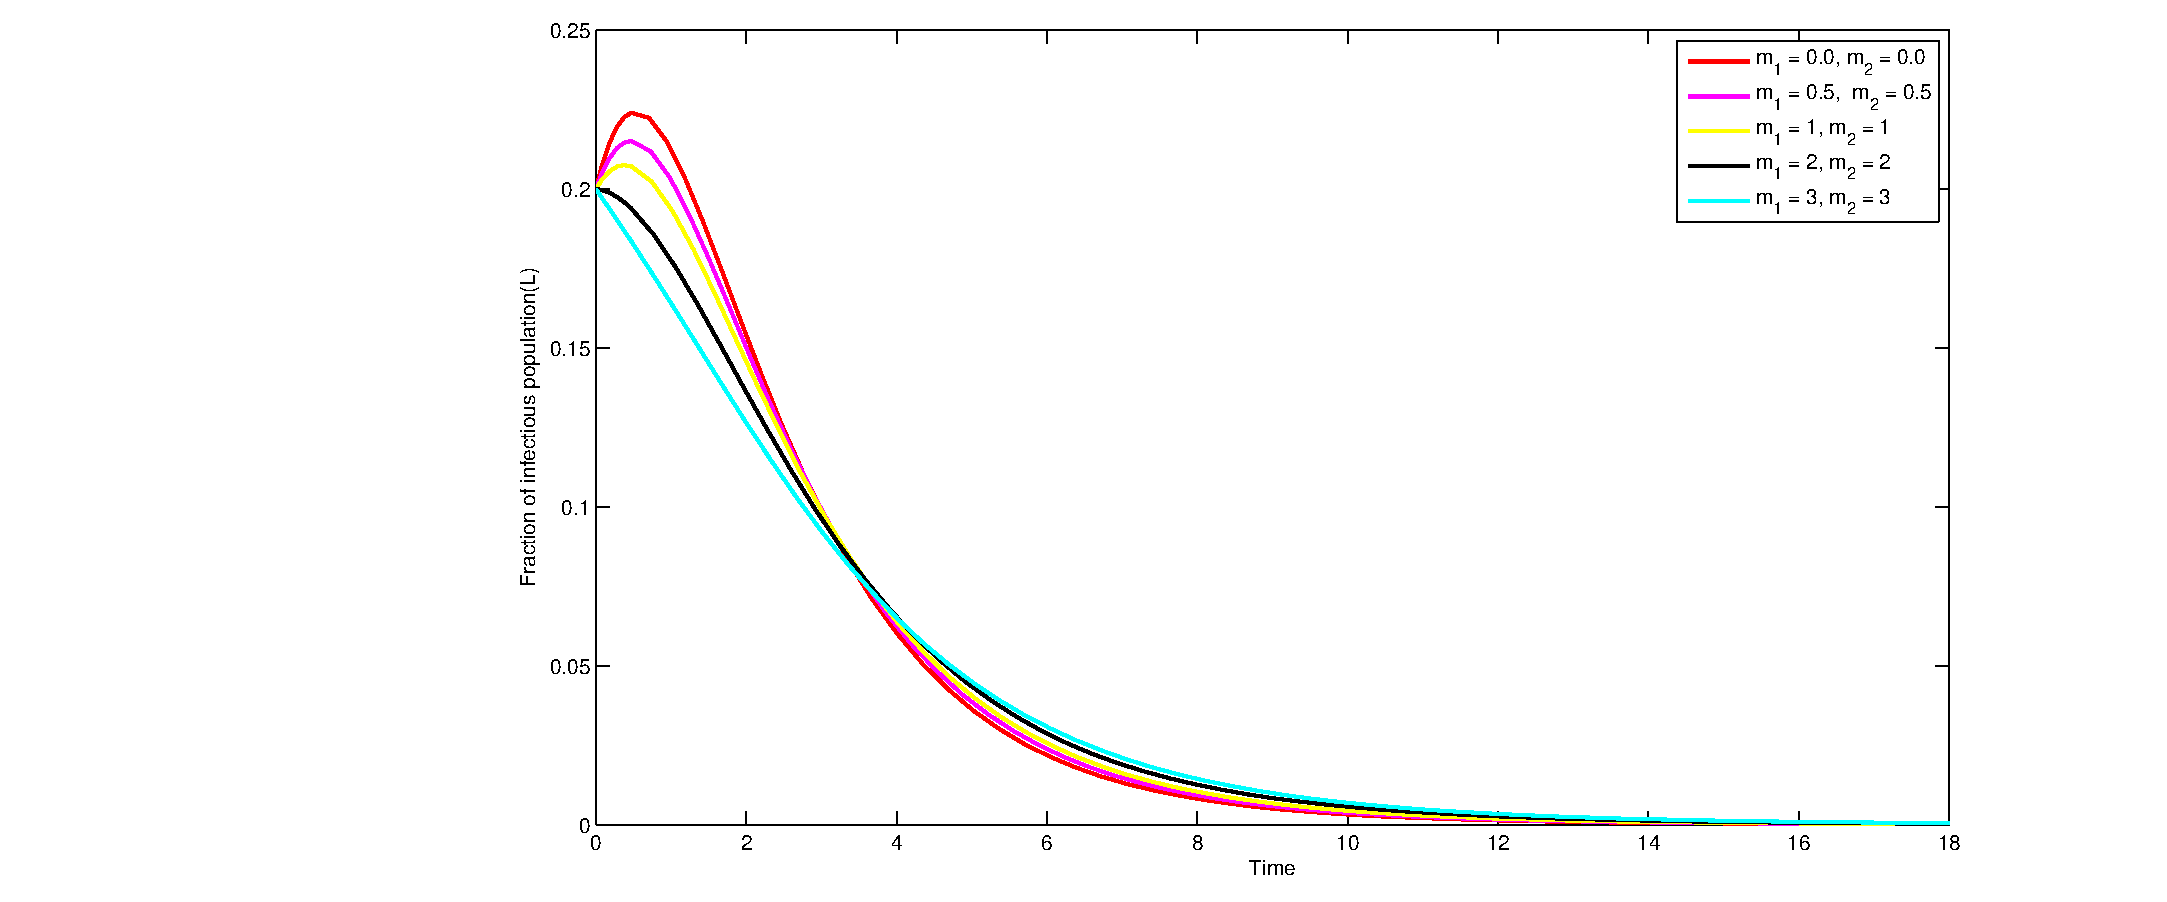
\includegraphics[width=7.5in]{mL1.eps}\\
  \caption{Effect of m on L when $R_0<1$}\label{fig:c2}
\end{figure}
\end{flushleft}
\begin{flushleft}
\begin{figure}[h!]
\centering
  % Requires \usepackage{graphicx}
  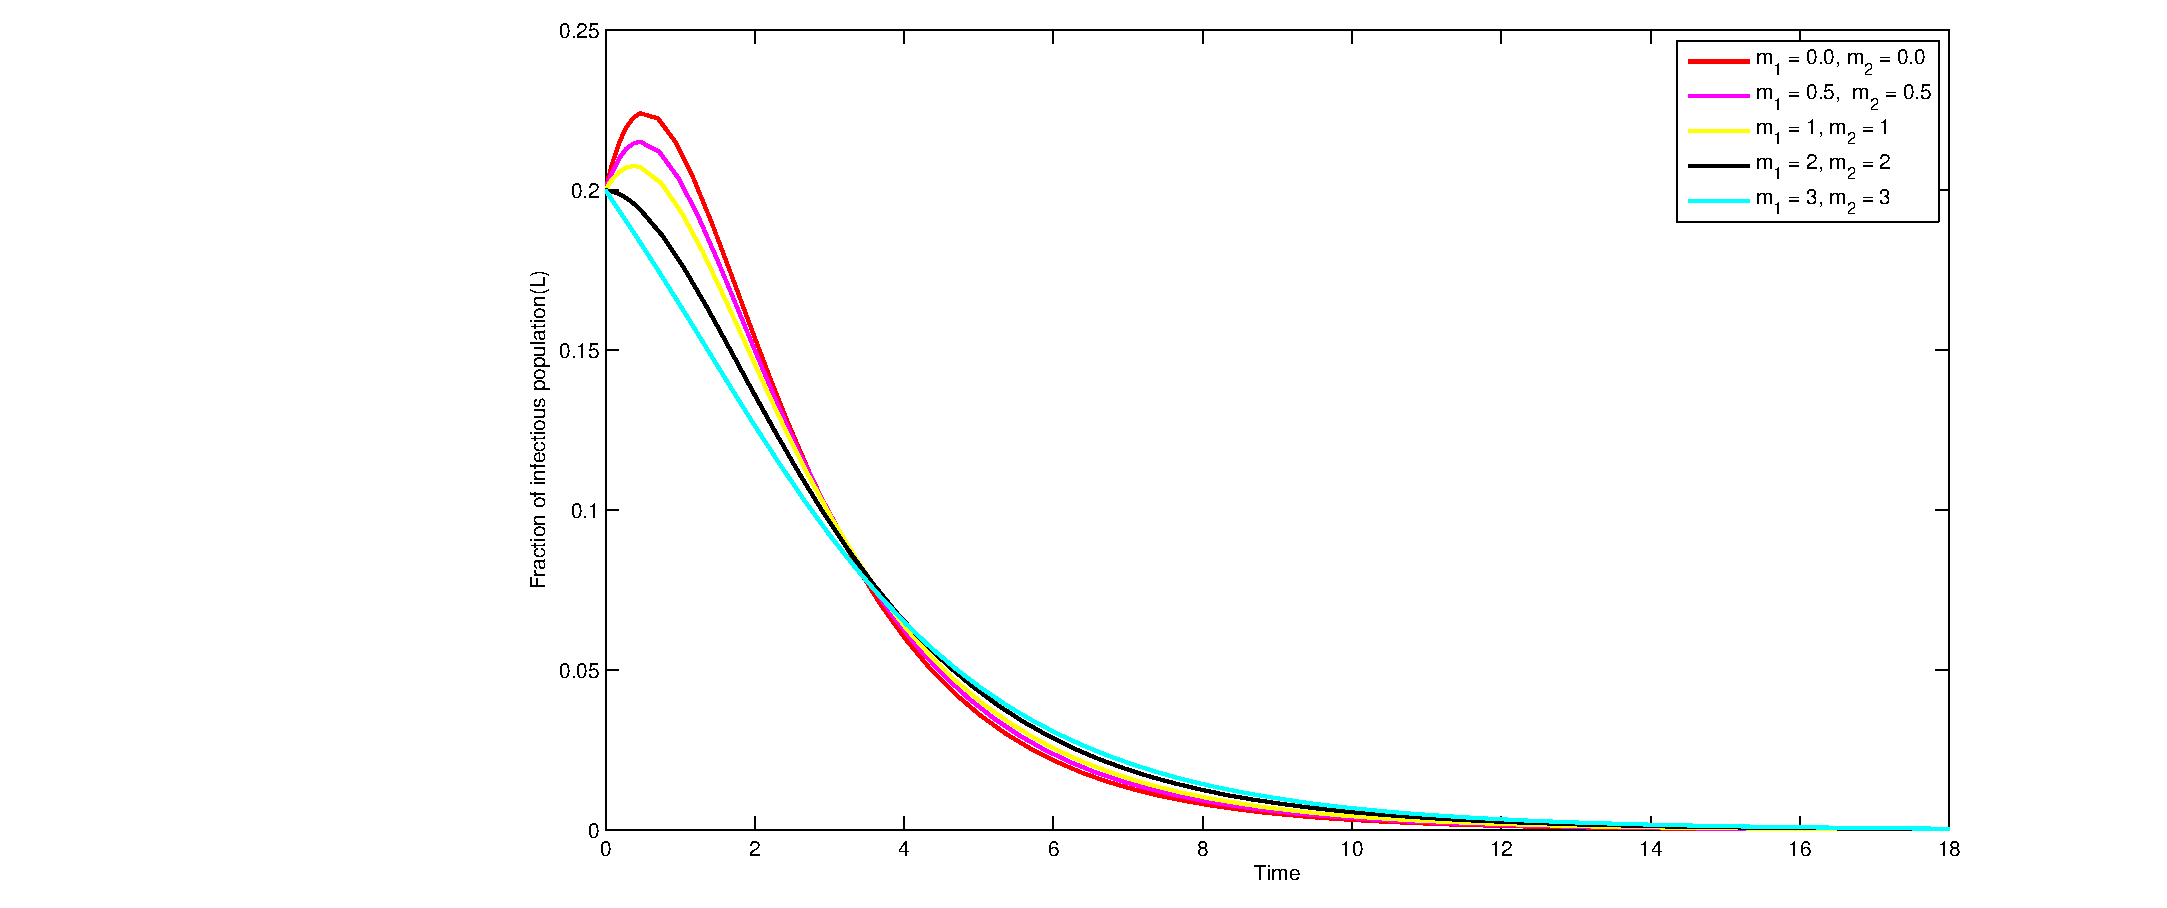
\includegraphics[width=7.5in]{mL2.eps}\\
  \caption{Effect of m on L when $R_0>1$}\label{fig:d2}
\end{figure}
\end{flushleft}

%\begin{figure}[h!]
%\centering
%\subfigure[Effect of m on B when $R_0<1$]{\label{fig:a2}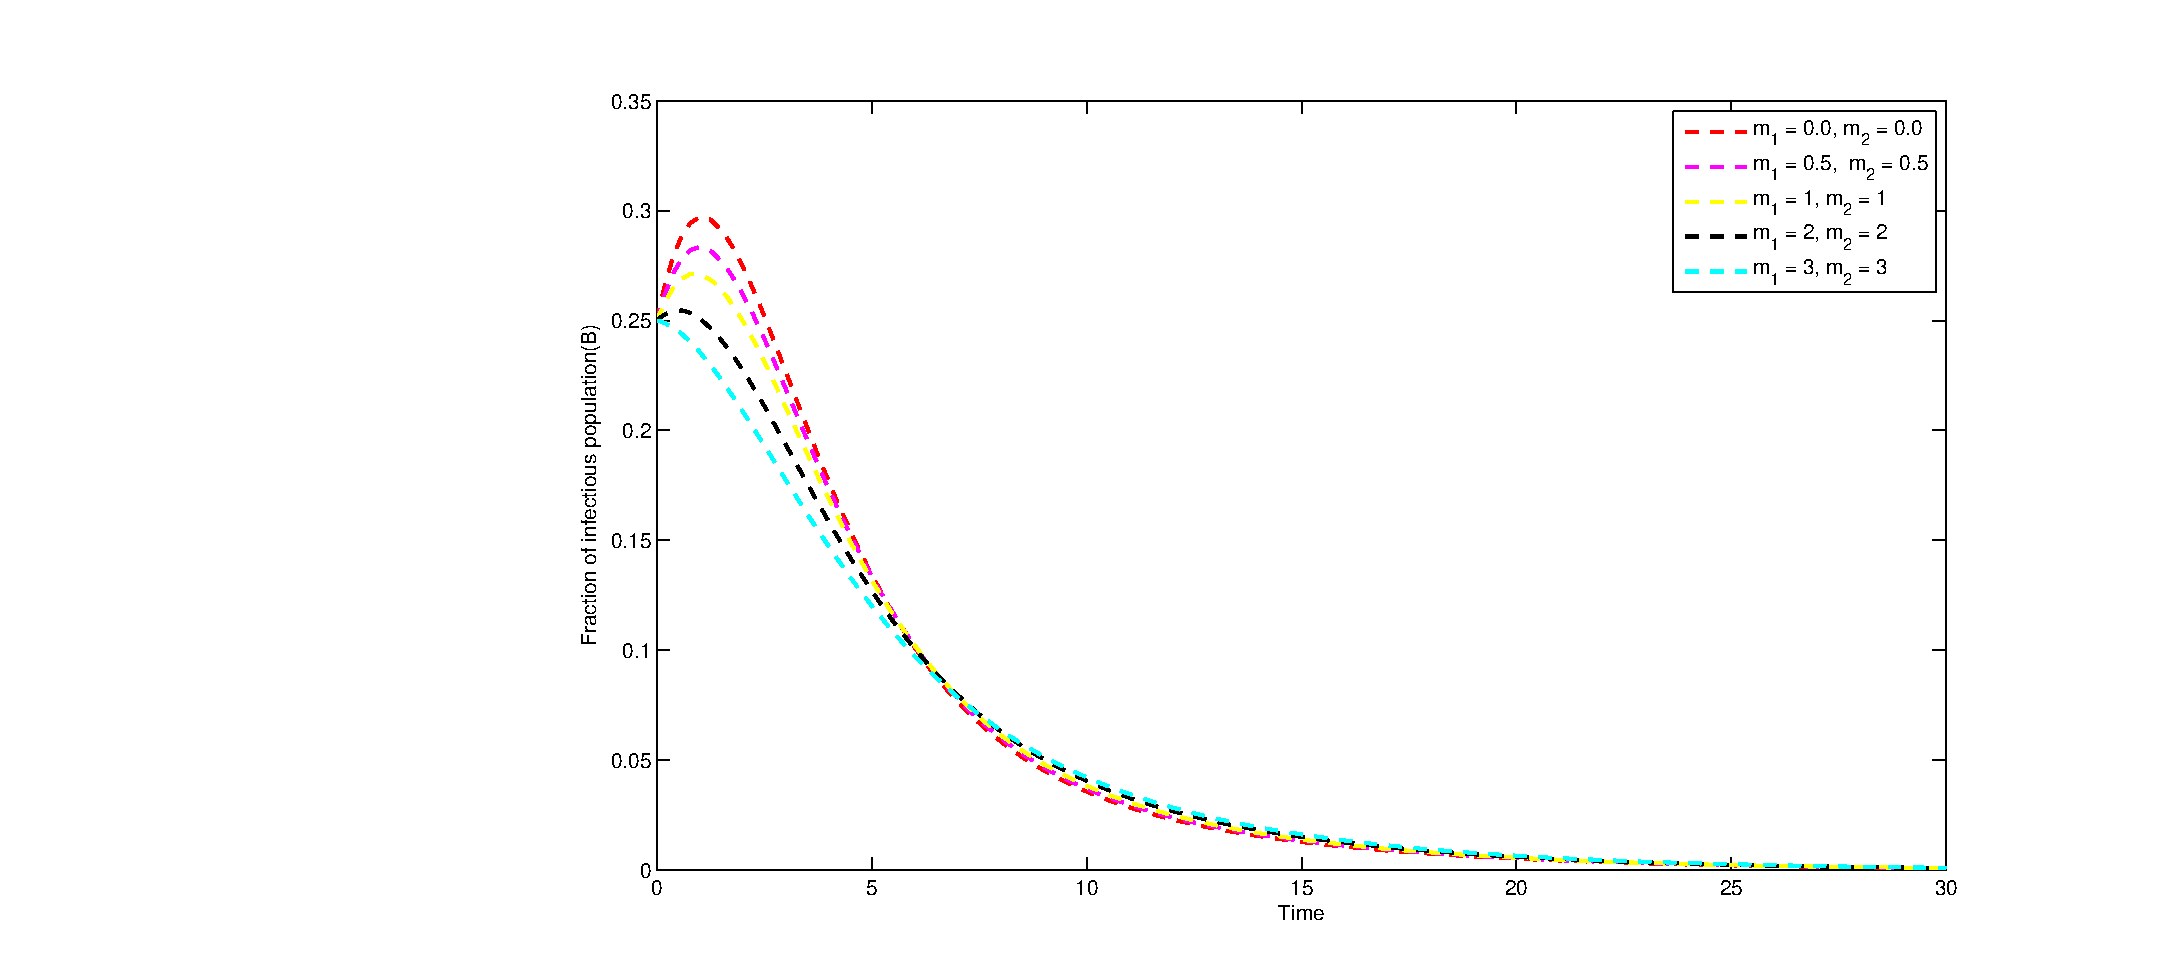
\includegraphics[width=7in,height=3.5in clip=true]{mB1.eps}}
%\end{figure}
%\begin{figure}[h!]
%\centering
%\subfigure[Effect of m on B when $R_0>1$]{\label{fig:b2}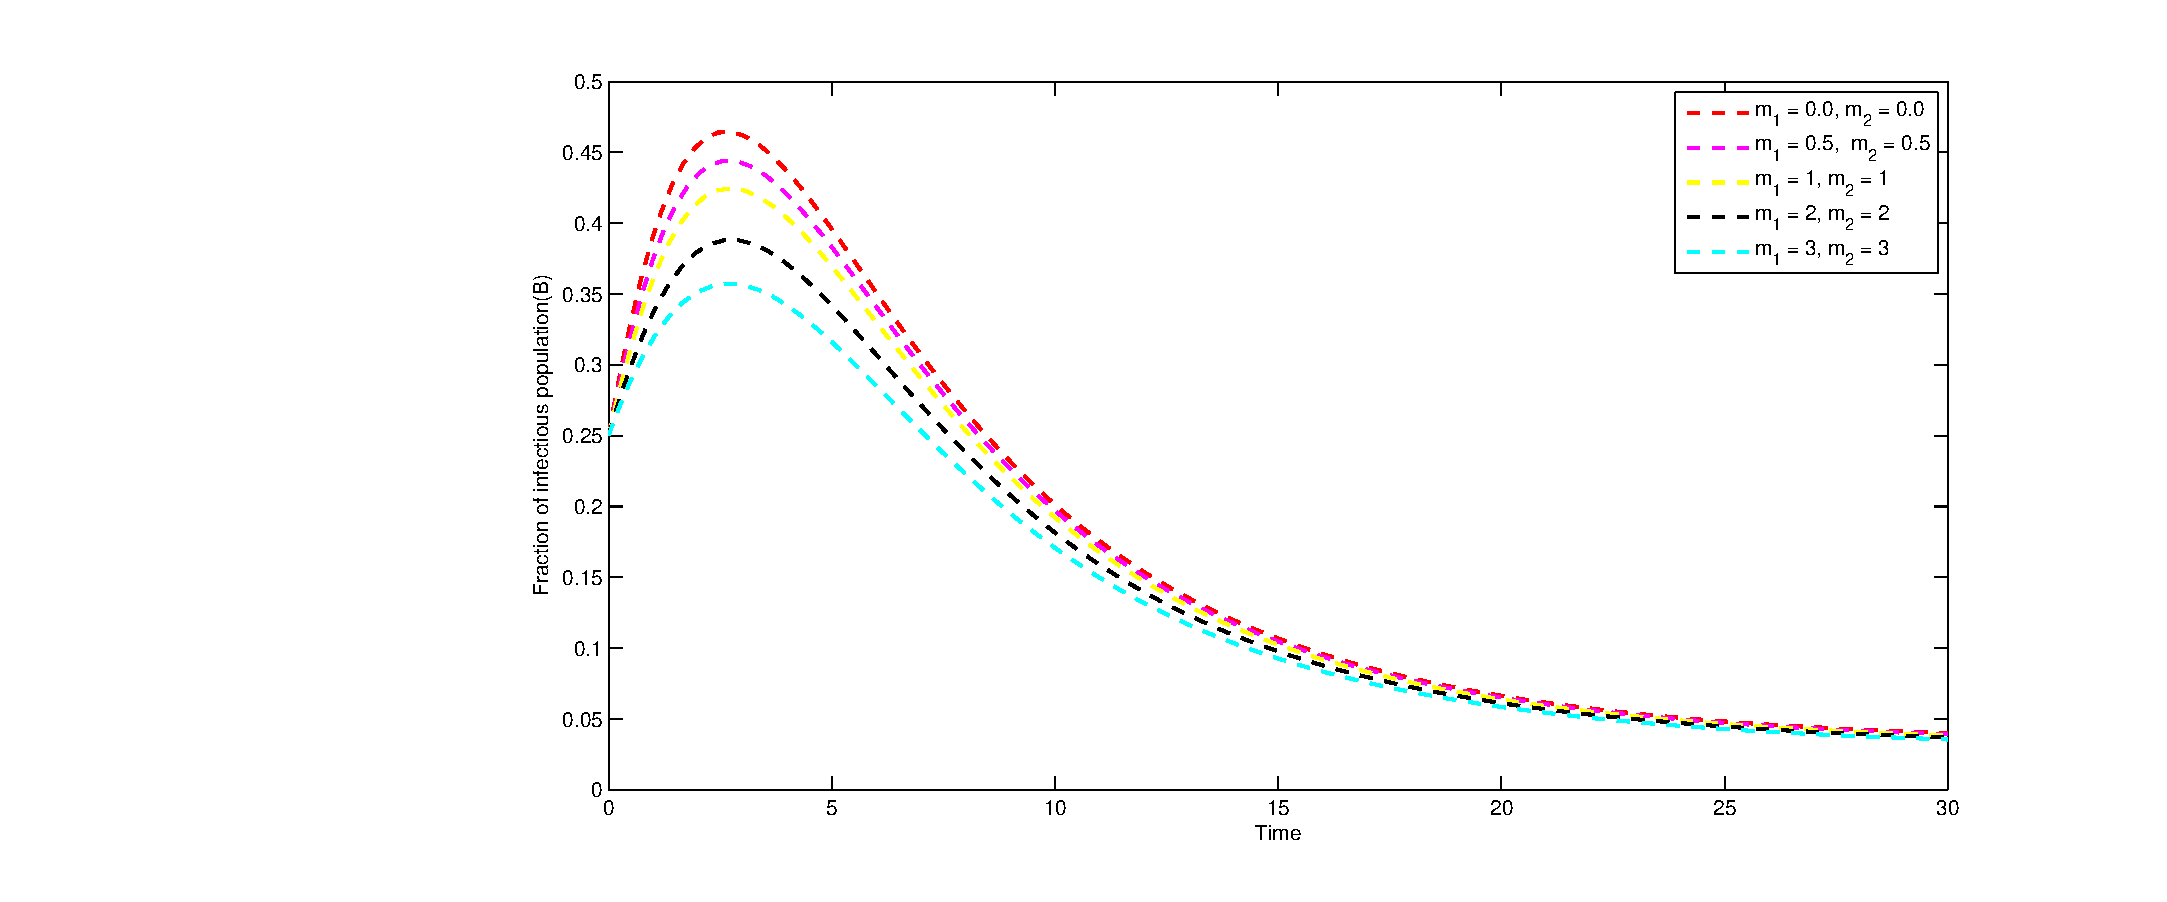
\includegraphics[width=7in, clip=true]{mB2.eps}}
%\end{figure}
%\newpage
%\begin{figure}[h!]
%\centering
%\subfigure[Effect of m on L when $R_0<1$]{\label{fig:c2}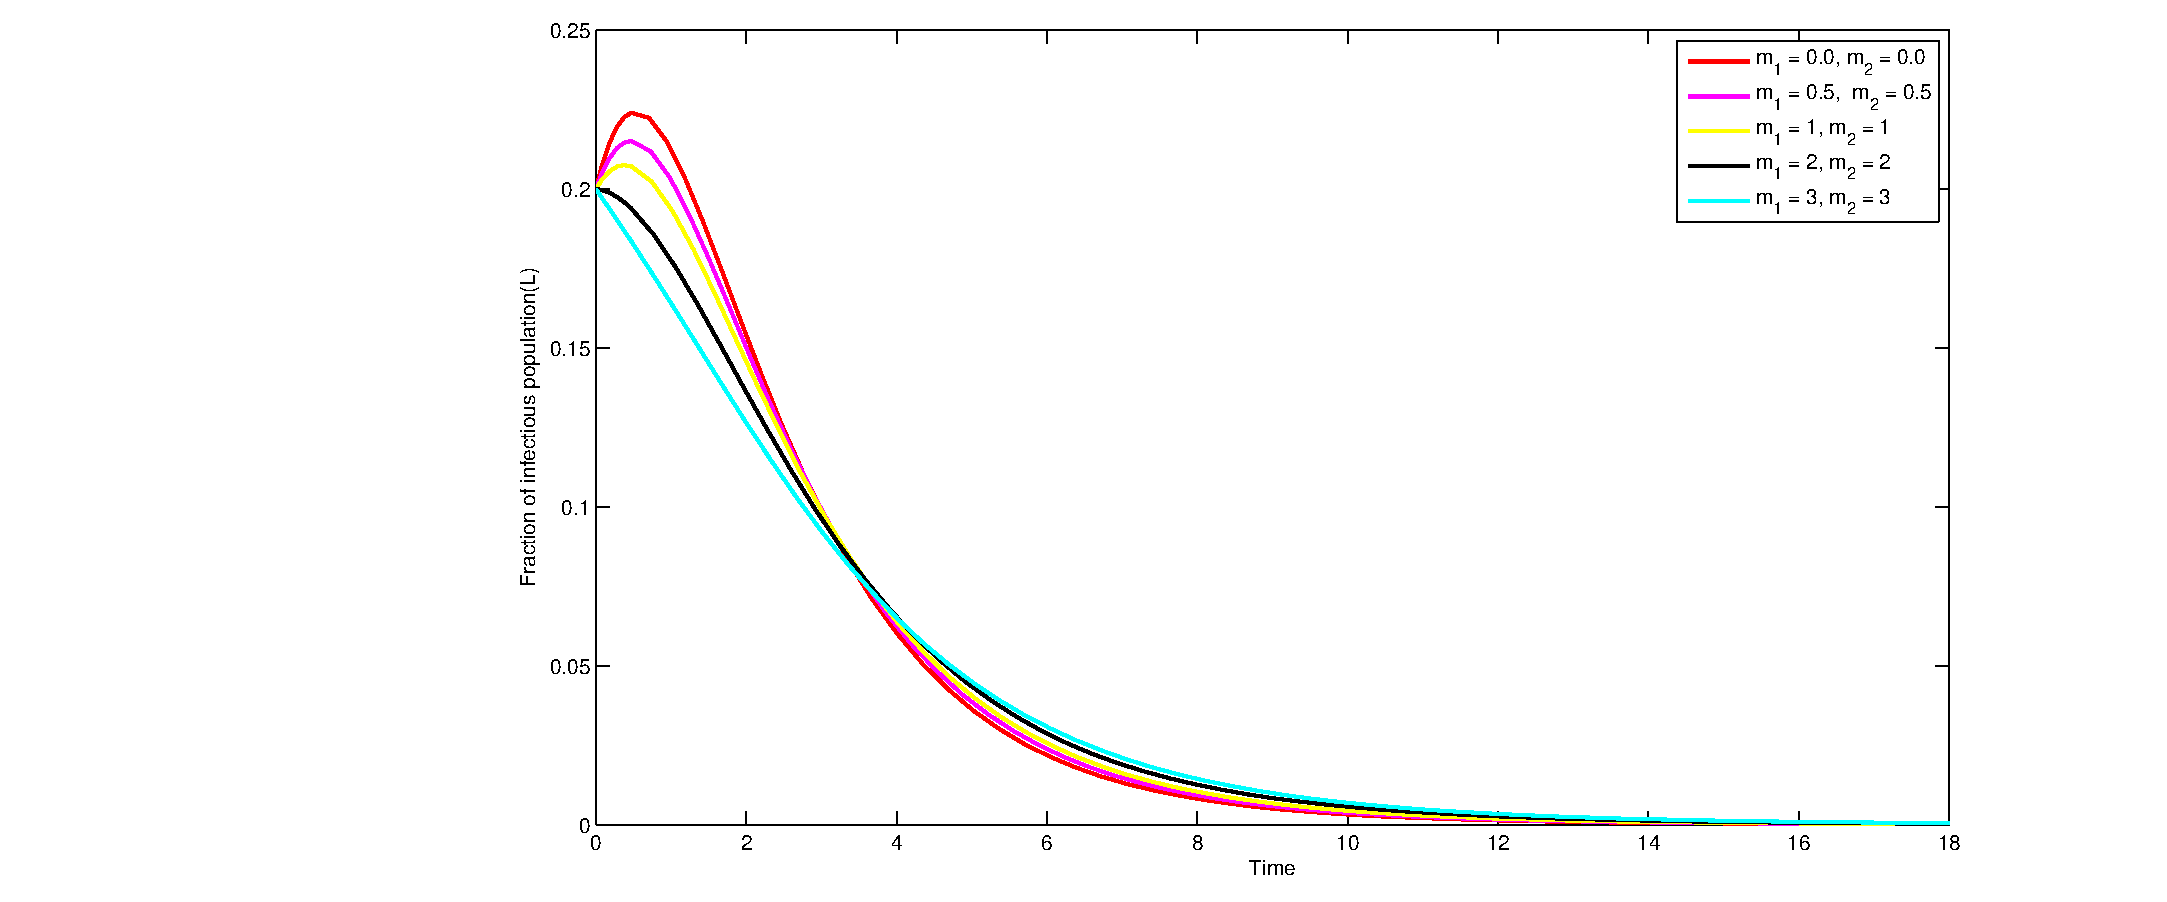
\includegraphics[width=7in, clip=true]{mL1.eps}}
%\end{figure}
%\begin{figure}[h!]
%\centering
%\subfigure[Effect of m on L when $R_0>1$]{\label{fig:d2}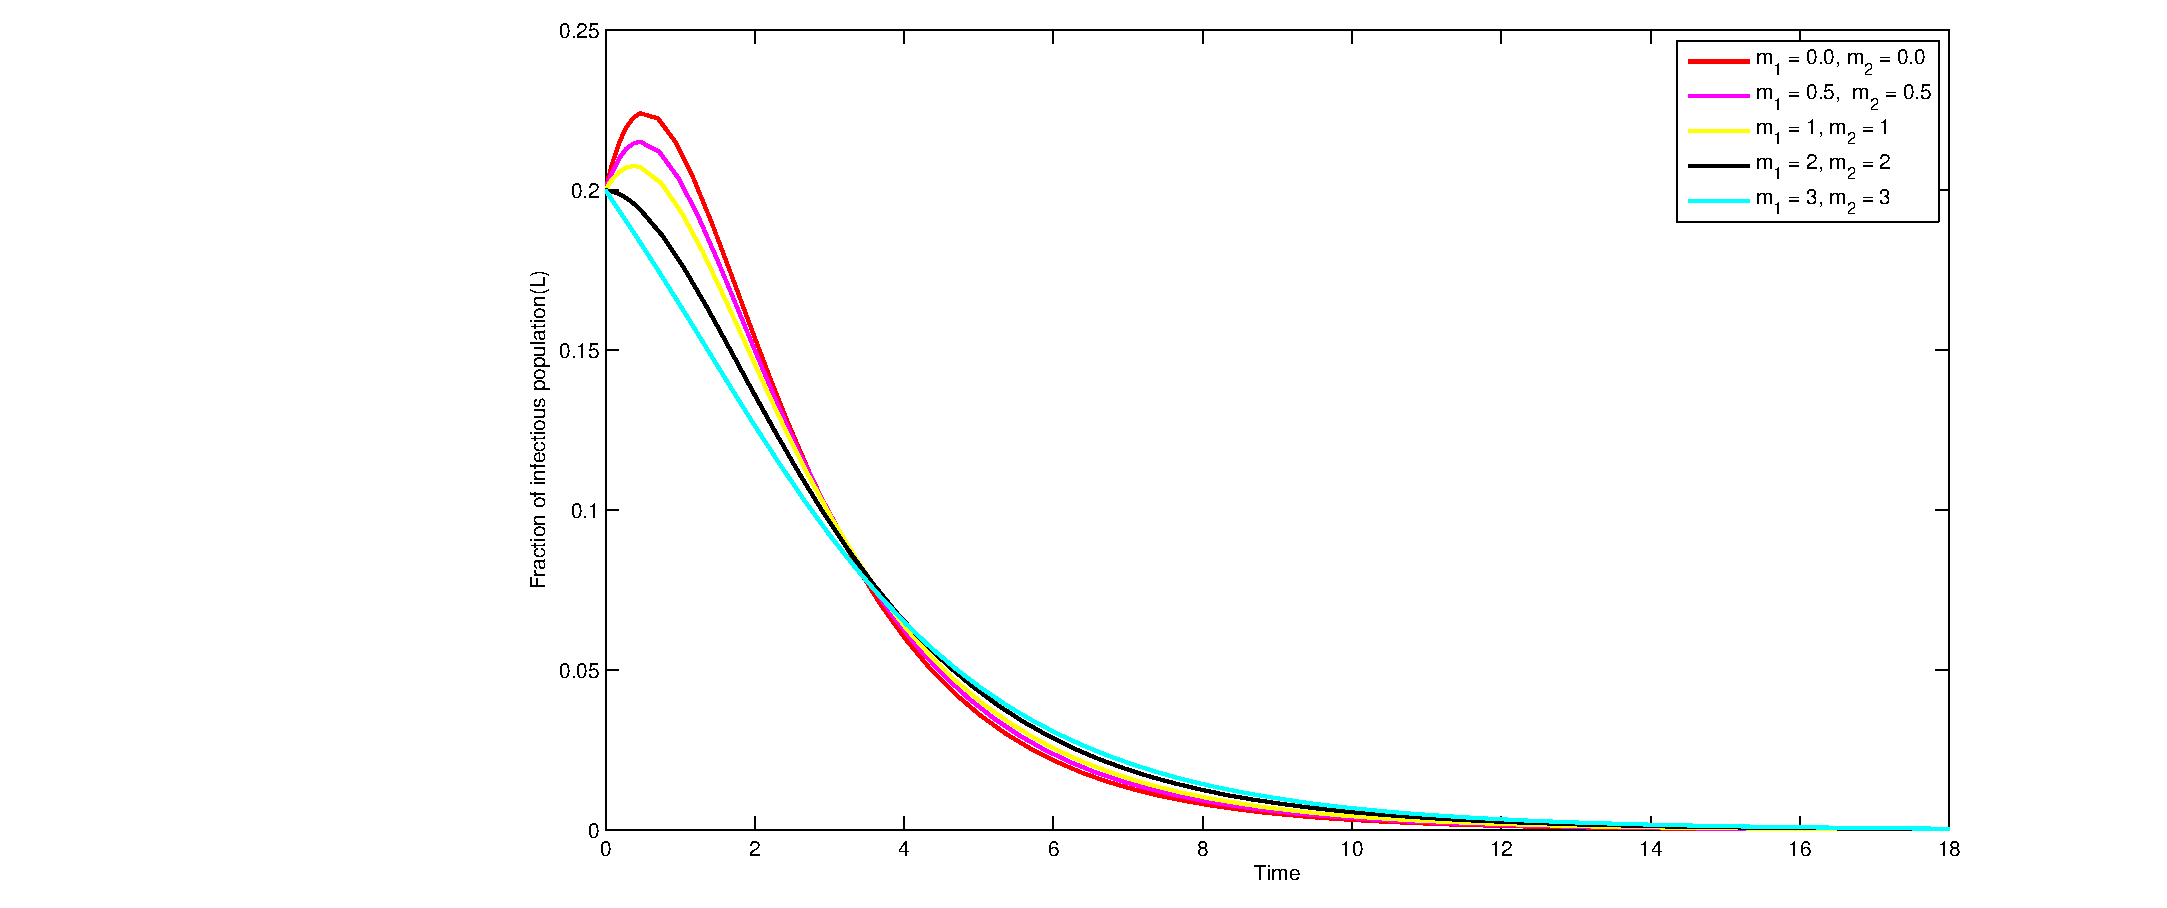
\includegraphics[width=7in, clip=true]{mL2.eps}}
%\caption{Effect of $m$ on fraction of infectious population}
%\end{figure}

\newpage
\section{Sensitivity Analysis:}
Normalized forward sensitivity index is used for the sensitivity analysis of basic reproduction number. Sensitivity indices enable us to quantify the relative change in a state variable with respect to a slight change in the system parameter.
The ratio of the relative change in the variable to the relative change in the particular system parameter is known as the normalized forward sensitivity index of the variable to that parameter. The sensitivity index may also be expressed using partial derivatives \citep{chitnis2008determining}. Let p is a parameter and $u$ is the function of $p$, a small perturbation $\delta_p$ to the parameter $p$ and the corresponding change in $u$ as $\delta_u$:
\[
\delta_u = u(p+\delta_p) - u(p)=\frac{u(p+\delta_p) - u(p)}{\delta_p}.\delta_p \approx \delta_p\frac{\partial u}{\partial p}.
\]
The normalized forward sensitivity index of a variable, $u$, that depends on a parameter, $p$, is defined as:
\[
 \varUpsilon^u_p = \frac{\partial u}{\partial p} \times \frac{p}{u}.
\]
Estimation and measurement of most sensitive parameter has to be done carefully, because a small change in the parameter will tend to relatively huge quantitative change. However, estimation of less sensitive parameter does not require as much effort,
since a small change in the parameter will not lead to huge change in the quantity.
With respect to each parameter, we derived analytical expressions for sensitivity index of $R_{0}$. The normalized
sensitivity indices for parameters are obtained as given in the following table.\\
\noindent The sensitivity indices of the basic reproduction numbers $R_{01}, R_{02}, R_{03}$ and  $R_{04}$
for all the parameter sets are listed below:\\
\newpage
\noindent 1. Normalized sensitivity indices for different parameter sets with respect to $R_{01}$  are shown in the table: \ref{T2}.\\
\begin{table}
\centering
    \begin{tabular}{|p{3cm}|p{1.6cm}|p{1.6cm}|p{1.6cm}|p{1.6cm}|p{1.6cm}|p{1.6cm}|p{1.6cm}|}
    \hline
               Parameters      & \textbf{$\varUpsilon^{{{\cal R}}_{01}}_{y_j}$ Set 1} & \textbf{$\varUpsilon^{{{\cal R}}_{01}}_{y_j}$ Set 2} & \textbf{$\varUpsilon^{{{\cal R}}_{01}}_{y_j}$ Set 3} & \textbf{$\varUpsilon^{{{\cal R}}_{01}}_{y_j}$ Set 4} & \textbf{$\varUpsilon^{{{\cal R}}_{01}}_{y_j}$ Set 5} & \textbf{$\varUpsilon^{{{\cal R}}_{01}}_{y_j}$ Set 6} \\
            \hline
  $\boldsymbol {\beta_{1}} $                 & 0 & 0.999 & 0 & 0 & 0 & 0  \\
  $\boldsymbol {\beta_{2}} $      & 0.999 & 0 & 0 & 0.999 & 0.999 & 0.9999  \\
  \textbf {k}       & 0 & 0 & 0 & 0 & 0 & 0  \\
  \textbf{c}                & 0 & 0 & 0 & 0 & 0 & 0  \\
  $\boldsymbol{\alpha}$          & 0 & 0 & 0 & 0 & 0 & 0  \\
  $\mathbf {d _{2} }$           & -0.47 & -0126 & 0 & -0.499 & -0.446 & -0.72  \\
  $\boldsymbol{\epsilon}$          & 0 & -0.476 & 0 & 0 & 0 & 0  \\
  $\boldsymbol{\gamma}$                & -0.529 & 0 & 0 & -0.499 & -0.553 & -0.285  \\
  $\boldsymbol{\delta}$        & 0 & -0.396 & 0 & 0 & 0 & 0  \\
  \textbf{f}           & 0 & 0 & 0 & 0 & 0 & 0  \\
  $\boldsymbol {\beta_{3}}$          & 0 & 0 & 0 & 0 & 0 & 0  \\
  $\boldsymbol {\beta_{4}}$             & 0 & 0 & 0.99 & 0 & 0 & 0  \\
  $\mathbf{f_{1} } $         & 0 & 0 & 0 & 0 & 0 & 0  \\
  $\mathbf{k_{1} }  $        & 0 & 0 & 0 & 0 & 0 & 0  \\
  $\mathbf{c_{1} } $         & 0 & 0 & 0 & 0 & 0 & 0  \\
  $\boldsymbol {\alpha_{1}}$          & 0 & 0 & 0 & 0 & 0 & 0  \\
  $\mathbf{d_{3}}$          & 0 & 0 & -0.499 & 0 & 0 & 0  \\
  $\boldsymbol {\gamma_{1}}$          & 0 & 0 & -0.499 & 0 & 0 & 0  \\
  $\boldsymbol {\delta_{1}}$         & 0 & 0 & 0 & 0 & 0 & 0  \\
  $\boldsymbol {\epsilon_{1}}$          & 0 & 0 & 0 & 0 & 0 & 0  \\
  \hline
    \end{tabular}
\caption{Normalized sensitivity indices for different parameter sets with respect to $R_{01}$}\label{T2}
\end{table}
\noindent We observed that $\beta_{1}, \beta_{2}$ and $\beta_{4}$ are highly sensitive. $d_{2}, \epsilon, \delta, \gamma, d_{3}$, and $\gamma_{1}$ are moderately sensitive and $k, c, \alpha,f, \beta_{3}, f_{1}, k_{1}, c_{1}, \alpha_{1}, \delta_{1}$  and $\epsilon_{1}$ are independent of $R_{01}$. For example $\varUpsilon^{{{\cal R}}_{01}}_{d_{2}}$ for set 1 = -0.47, hence,
increasing (decreasing) $d_{2}$ by 1\% will decrease (increase) $R_{01}$  by 0.47\%.
\newpage
\noindent 2. Normalized sensitivity indices for different parameter sets with respect to $R_{02}$ are shown in the table: \ref{T3}.\\
\begin{table}
\centering
    \begin{tabular}{|p{3cm}|p{1.6cm}|p{1.6cm}|p{1.6cm}|p{1.6cm}|p{1.6cm}|p{1.6cm}|p{1.6cm}|}
    \hline
               Parameters      & \textbf{$\varUpsilon^{{{\cal R}}_{02}}_{y_j}$ Set 1} & \textbf{$\varUpsilon^{{{\cal R}}_{02}}_{y_j}$ Set 2} & \textbf{$\varUpsilon^{{{\cal R}}_{02}}_{y_j}$ Set 3} & \textbf{$\varUpsilon^{{{\cal R}}_{02}}_{y_j}$ Set 4} & \textbf{$\varUpsilon^{{{\cal R}}_{02}}_{y_j}$ Set 5} & \textbf{$\varUpsilon^{{{\cal R}}_{02}}_{y_j}$ Set 6} \\
            \hline
  $\boldsymbol {\beta_{1}} $                 & 0 & 0.999 & 0 & 0 & 0 & 0  \\
  $\boldsymbol {\beta_{2}} $      & 0.999 & 0 & 0 & 0.999 & 0.999 & 0.9999  \\
  $\boldsymbol{\alpha}$          & 0 & 0 & 0 & 0 & 0 & 0  \\
  $\mathbf {d _{2} }$           & -0.47 & -0.126 & -0.49 & -0.49 & -0.44 & -0.71  \\
  $\boldsymbol{\epsilon}$           & 0 & -0.476 & 0 & 0 & 0 & 0  \\
  $\boldsymbol{\gamma}$               & -0.529 & 0 & -0.499 & -0.499 & -0.533 & -0.285  \\
  $\boldsymbol{\delta}$        & 0 & -0.396 & 0 & 0 & 0 & 0  \\
  \textbf{f}          & 0 & 0 & 0 & 0 & 0 & 0  \\
  $\boldsymbol {\beta_{3}}$          & 0 & 0 & 0 & 0 & 0 & 0  \\
  $\boldsymbol {\beta_{4}}$             & 0 & 0 & 0 & 0 & 0 & 0  \\
  $\mathbf{f_{1} } $         & 0 & 0 & 0 & 0 & 0 & 0  \\
  $\mathbf{k_{1} }  $        & 0 & 0 & 0 & 0 & 0 & 0  \\
  $\mathbf{c_{1} } $         & 0 & 0 & 0 & 0 & 0 & 0  \\
  $\boldsymbol {\alpha_{1}}$          & 0 & 0 & 0 & 0 & 0 & 0  \\
  $\mathbf{d_{3}}$          & 0 & 0 & 0 & 0 & 0 & 0  \\
  $\boldsymbol {\gamma_{1}}$          & 0 & 0 & 0 & 0 & 0 & 0  \\
  $\boldsymbol {\delta_{1}}$         & 0 & 0 & 0 & 0 & 0 & 0  \\
  $\boldsymbol {\epsilon_{1}}$          & 0 & 0 & 0 & 0 & 0 & 0  \\
  \hline
    \end{tabular}
\caption{Normalized sensitivity indices for different parameter sets with respect to $R_{02}$}\label{T3}
\end{table}
\noindent We observed that $\beta_{1}$ and $\beta_{2}$  are highly sensitive. $d_{2}, \epsilon, \delta,$ and $ \gamma$, are moderately sensitive and $k, c, \alpha,f, \beta_{3}, f_{1}, k_{1}, c_{1}, \alpha_{1}, \delta_{1},\beta_{4}$  and $\epsilon_{1}$ are independent of $R_{02}$ . For example $\varUpsilon^{{{\cal R}}_{02}}_{\beta_{2}}$ for set 1 = 0.99, hence, increasing (decreasing) $d_{2}$ by 1\%  will increase (decrease) $R_{02}$  by 0.99\% .
\newpage
\noindent 3. Normalized sensitivity indices for different parameter sets with respect to $R_{03}$ are shown in the table: \ref{T4}.\\
\begin{table}
\centering
    \begin{tabular}{|p{3cm}|p{1.6cm}|p{1.6cm}|p{1.6cm}|p{1.6cm}|p{1.6cm}|p{1.6cm}|p{1.6cm}|}
    \hline
               Parameters      & \textbf{$\varUpsilon^{{{\cal R}}_{03}}_{y_j}$ Set 1} & \textbf{$\varUpsilon^{{{\cal R}}_{03}}_{y_j}$ Set 2} & \textbf{$\varUpsilon^{{{\cal R}}_{03}}_{y_j}$ Set 3} & \textbf{$\varUpsilon^{{{\cal R}}_{03}}_{y_j}$ Set 4} & \textbf{$\varUpsilon^{{{\cal R}}_{03}}_{y_j}$ Set 5} & \textbf{$\varUpsilon^{{{\cal R}}_{03}}_{y_j}$ Set 6} \\
            \hline
  $\boldsymbol {\beta_{1}} $                 & 0 & 0 & 0 & 0 & 0 & 0  \\
  $\boldsymbol {\beta_{2}} $      & 0 & 0 & 0 & 0 & 0.99 & 0.99  \\
  \textbf {k}       & 0 & 0 & 0 & 0 & -0.99 & -0.99  \\
  \textbf{c}                & 0 & 0 & 0 & 0 & 0.99 & 0.99  \\
  $\boldsymbol{\alpha}$          & 0 & 0 & 0 & 0 & 0 & 0  \\
  $\mathbf {d _{2} }$           & 0 & 0 & 0 & 0 & -0.44 & -0.71  \\
  $\boldsymbol{\epsilon}$          & 0 & 0 & 0 & 0 & 0 & 0  \\
  $\boldsymbol{\gamma}$                & 0 & 0 & 0 & 0 & -0.55 & -0.28  \\
  $\boldsymbol{\delta}$        & 0 & 0 & 0 & 0 & 0 & 0  \\
  \textbf{f}           & 0 & 0 & 0 & 0 & 0 & 0  \\
  $\boldsymbol {\beta_{3}}$          & 0 & 0.99 & 0 & 0 & 0 & 0  \\
  $\boldsymbol {\beta_{4}}$             & 0.99 & 0 & 0.99 & 0.99 & 0 & 0  \\
  $\mathbf{f_{1} } $         & 0 & 0 & 0 & 0 & 0 & 0  \\
  $\mathbf{k_{1} }  $        & 0 & 0 & 0 & 0 & 0 & 0  \\
  $\mathbf{c_{1} } $         & 0 & 0 & 0 & 0 & 0 & 0  \\
  $\boldsymbol {\alpha_{1}}$          & 0 & 0 & 0 & 0 & 0 & 0  \\
  $\mathbf{d_{3}}$          & -0.58 & -0.09 & -0.499 & -0.499 & 0 & 0  \\
  $\boldsymbol {\gamma_{1}}$          & -0.411 & 0 & -0.499 & -0.499 & 0 & 0  \\
  $\boldsymbol {\delta_{1}}$         & 0 & -0.399 & 0 & 0 & 0 & 0  \\
  $\boldsymbol {\epsilon_{1}}$          & 0 & -0.499 & 0 & 0 & 0 & 0  \\
  \hline
    \end{tabular}
\caption{Normalized sensitivity indices for different parameter sets with respect to $R_{03}$}\label{T4}
\end{table}
\noindent We observed that $\beta_{2}$, $\beta_{3}$, $\beta_{4}$, $k$ and $c$ are highly sensitive, $d_{2}, \epsilon_{1}, \gamma, \gamma_{1}$ and $\delta_{1},$ and , are moderately sensitive and $\alpha, f,
\delta, \beta_{1}, f_{1}, k_{1}, c_{1}$ and $\alpha_{1}$ are independent of $R_{03}$ . For example $\varUpsilon^{{{\cal R}}_{03}}_{\gamma}$ for set 5 = -0.55, hence, increasing (decreasing) $d_{2}$ by 1\% will decrease(increase) $R_{03}$ by 0.55\% .
\newpage
\noindent 4. Normalized sensitivity indices for different parameter sets with respect to $R_{04}$ are shown in the table: \ref{T5}.\\
\begin{table}
\centering
    \begin{tabular}{|p{3cm}|p{1.6cm}|p{1.6cm}|p{1.6cm}|p{1.6cm}|p{1.6cm}|p{1.6cm}|p{1.6cm}|}
    \hline
               Parameters      & \textbf{$\varUpsilon^{{{\cal R}}_{04}}_{y_j}$ Set 1} & \textbf{$\varUpsilon^{{{\cal R}}_{04}}_{y_j}$ Set 2} & \textbf{$\varUpsilon^{{{\cal R}}_{04}}_{y_j}$ Set 3} & \textbf{$\varUpsilon^{{{\cal R}}_{04}}_{y_j}$ Set 4} & \textbf{$\varUpsilon^{{{\cal R}}_{04}}_{y_j}$ Set 5} & \textbf{$\varUpsilon^{{{\cal R}}_{04}}_{y_j}$ Set 6} \\
            \hline
  $\boldsymbol {\beta_{1}} $                 & 0 & 0.99 & 0 & 0 & 0 & 0  \\
  $\boldsymbol {\beta_{2}} $      & 0.99 & 0 & 0.99 & 0.99 & 0.99 & 0.99 \\
  \textbf {k}       & -0.99 & -0.99 & -0.99 & -0.99 & -0.99 & -0.99  \\
  \textbf{c}               & -0.99 & -0.99 & -0.99 & -0.99 & -0.99 & -0.99  \\
  $\boldsymbol{\alpha}$          & 0 & 0 & 0 & 0 & 0 & 0  \\
  $\mathbf {d _{2} }$           & -0.47 & -0.12 & -0.49 & -0.49 & -0.44 & -0.71  \\
  $\boldsymbol{\epsilon}$          & 0 & -0.47 & 0 & 0 & 0 & 0  \\
  $\boldsymbol{\gamma}$                & -0.52 & 0 & -0.49 & -0.49 & -0.55 & -0.28  \\
  $\boldsymbol{\delta}$        & 0 & -0.39 & 0 & 0 & 0 & 0  \\
  \textbf{f}           & 0 & 0 & 0 & 0 & 0 & 0  \\
  $\boldsymbol {\beta_{3}}$          & 0 & 0 & 0 & 0 & 0 & 0  \\
  $\boldsymbol {\beta_{4}}$             & 0 & 0 & 0 & 0 & 0 & 0  \\
  $\mathbf{f_{1} } $         & 0 & 0 & 0 & 0 & 0 & 0  \\
  $\mathbf{k_{1} }  $        & 0 & 0 & 0 & 0 & 0 & 0  \\
  $\mathbf{c_{1} } $         & 0 & 0 & 0 & 0 & 0 & 0  \\
  $\boldsymbol {\alpha_{1}}$          & 0 & 0 & 0 & 0 & 0 & 0  \\
  $\mathbf{d_{3}}$          & 0 & 0 & 0 & 0 & 0 & 0  \\
  $\boldsymbol {\gamma_{1}}$          & 0 & 0 & 0 & 0 & 0 & 0  \\
  $\boldsymbol {\delta_{1}}$         & 0 & 0 & 0 & 0 & 0 & 0  \\
  $\boldsymbol {\epsilon_{1}}$          & 0 & 0 & 0 & 0 & 0 & 0  \\
  \hline
    \end{tabular}
\caption{Normalized sensitivity indices for parameters set with respect to $R_{04}$}\label{T5}
\end{table}
\noindent We observed that $\beta_{1}$, $\beta_{2}$, $k$ and $c$ are highly sensitive. $d_{2}, \epsilon, \gamma$ and $\delta$  are moderately sensitive and $\alpha,\alpha_{1}, f,\beta_{3},\beta_{4},\delta_{1},\gamma_{1}, \beta_{1},d_{3}, f_{1}, k_{1}, c_{1}$ and $\epsilon_{1}$ are independent of $R_{04}$. For example $\varUpsilon^{{{\cal R}}_{04}}_{k}$ for set 1 = -0.99, therefore, increasing (decreasing) $d_{2}$ by 1\% will decrease(increase) $R_{04}$ by 0.99\%.




